% ******************************* PhD Thesis Template 
%**************************
% Please have a look at the README.md file for info on how to use the template

\documentclass[a4paper,21pt,times,numbered,print,index,customargin]{Classes/PhDThesisPSnPDF}
\usepackage{longtable}
\usepackage{titlesec}
\usepackage{adjustbox}
\usepackage{fixltx2e} 

% ********************************** Preamble **********************************
% Preamble: Contains packages and user-defined commands and settings
% ******************************************************************************
% ****************************** Custom Margin *********************************

% Add `custommargin' in the document class options to use this section
% Set {innerside margin / outerside margin / topmargin / bottom margin}  and
% other page dimensions
\ifsetCustomMargin
\RequirePackage[left=30mm,right=20mm,top=20mm,bottom=20mm]{geometry}
\setFancyHdr % To apply fancy header after geometry package is loaded
\fi

% *****************************************************************************
% ******************* Fonts (like different typewriter fonts etc.)*************

% Add `customfont' in the document class option to use this section

\ifsetCustomFont
  % Set your custom font here and use `customfont' in options. Leave empty to
  % load computer modern font (default LaTeX font).
  \RequirePackage{libertine}
\fi
\RequirePackage{dsfont} % Math font

% *****************************************************************************
% **************************** Custom Packages ********************************

\usepackage[inline]{enumitem}
\usepackage{hyperref}


% ************************* Algorithms and Pseudocode **************************

\RequirePackage{algpseudocode}
\RequirePackage{algorithm}


% ********************Captions and Hyperreferencing / URL **********************

% Captions: This makes captions of figures use a boldfaced small font.
%\RequirePackage[small,bf]{caption}

\RequirePackage[labelsep=space,tableposition=top,font=small,
justification=justified]{caption}
%\renewcommand{\figurename}{Fig.} %to support older versions of captions.sty


% *************************** Graphics and figures *****************************

%\usepackage{rotating}
%\usepackage{wrapfig}

% Uncomment the following two lines to force Latex to place the figure.
% Use [H] when including graphics. Note 'H' instead of 'h'
%\usepackage{float}
%\restylefloat{figure}

% Subcaption package is also available in the sty folder you can use that by
% uncommenting the following line
% This is for people stuck with older versions of texlive
%\usepackage{sty/caption/subcaption}
\usepackage{subcaption}
\captionsetup{compatibility=false}

% ********************************** Tables ************************************
\usepackage{booktabs} % For professional looking tables
%\usepackage{multirow}

%\usepackage{multicol}
%\usepackage{longtable}
%\usepackage{tabularx}


% ***************************** Math and SI Units ******************************

\usepackage{amsfonts}
\usepackage{amsmath}
\usepackage{amssymb}
\usepackage[per=slash]{siunitx} % use this package module for SI units
\usepackage{flexisym}
\usepackage{breqn}


% ******************************* Line Spacing *********************************

% Choose linespacing as appropriate. Default is one-half line spacing as per the
% University guidelines

% \doublespacing
% \onehalfspacing
% \singlespacing


% ************************ Formatting / Footnote *******************************

%\usepackage[perpage]{footmisc} %Range of footnote options

% *****************************************************************************
% *************************** Bibliography  and References ********************

\usepackage[noabbrev]{cleveref} %Referencing without need to 
\crefname{pluralequation}{equations}{eqns.}
\crefformat{equation}{#2eq.~#1#3}

\crefname{algocf}{alg.}{algs.}
\Crefname{algocf}{Algorithm}{Algorithms}


%explicitly state 
%fig /table

% Add `custombib' in the document class option to use this section
\ifuseCustomBib
%   \RequirePackage[square, sort, numbers, authoryear]{natbib} % CustomBib

% If you would like to use biblatex for your reference management, as opposed to the default `natbibpackage` pass the option `custombib` in the document class. Comment out the previous line to make sure you don't load the natbib package. Uncomment the following lines and specify the location of references.bib file

%\RequirePackage[backend=biber, style=authoryear-comp, 
%itestyle=authoryear-comp, sorting=nty, natbib=true, url=false]{biblatex}
%\bibliography{References/references} %Location of references.bib only for 
%biblatex

\fi

% changes the default name `Bibliography` -> `References'
%\renewcommand{\bibname}{References}


% *****************************************************************************
% *************** Changing the Visual Style of Chapter Headings ***************
% This section on visual style is from https://github.com/cambridge/thesis

% Uncomment the section below. Requires titlesec package.

%\RequirePackage{titlesec}
%\newcommand{\PreContentTitleFormat}{\titleformat{\chapter}[display]{\scshape\Large}
%{\Large\filleft{\chaptertitlename} \Huge\thechapter}
%{1ex}{}
%[\vspace{1ex}\titlerule]}
%\newcommand{\ContentTitleFormat}{\titleformat{\chapter}[display]{\scshape\huge}
%{\Large\filleft{\chaptertitlename} \Huge\thechapter}{1ex}
%{\titlerule\vspace{1ex}\filright}
%[\vspace{1ex}\titlerule]}
%\newcommand{\PostContentTitleFormat}{\PreContentTitleFormat}
%\PreContentTitleFormat


% ******************************************************************************
% ************************* User Defined Commands ******************************
% ******************************************************************************

% *********** To change the name of Table of Contents / LOF and LOT ************

%\renewcommand{\contentsname}{My Table of Contents}
%\renewcommand{\listfigurename}{My List of Figures}
%\renewcommand{\listtablename}{My List of Tables}


% ********************** TOC depth and numbering depth *************************

\setcounter{secnumdepth}{2}
\setcounter{tocdepth}{2}


% ******************************* Nomenclature *********************************

% To change the name of the Nomenclature section, uncomment the following line

%\renewcommand{\nomname}{Symbols}


% ********************************* Appendix ***********************************

% The default value of both \appendixtocname and \appendixpagename is `Appendices'. These names can all be changed via:

%\renewcommand{\appendixtocname}{List of appendices}
%\renewcommand{\appendixname}{Appndx}

% ******************************** Draft Mode **********************************

% Uncomment to disable figures in `draftmode'
%\setkeys{Gin}{draft=true}  % set draft to false to enable figures in `draft'

% These options are active only during the draft mode
% Default text is "Draft"
%\SetDraftText{DRAFT}

% Default Watermark location is top. Location (top/bottom)
%\SetDraftWMPosition{bottom}

% Draft Version - default is v1.0
%\SetDraftVersion{v1.1}

% Draft Text grayscale value (should be between 0-black and 1-white)
% Default value is 0.75
%\SetDraftGrayScale{0.8}

% ********************************** Listings **********************************
\usepackage{listings}
\usepackage{color}
\usepackage{xcolor}

\definecolor{light-gray}{gray}{0.95}
\lstdefinestyle{customcpp}{
  backgroundcolor=\color{light-gray},
  belowcaptionskip=1\baselineskip,
  breaklines=true,
  xleftmargin=\parindent,
  language=C++,
  numbers=left,
  numbersep=5pt, 
  numberstyle=\tiny\color{gray},
  showstringspaces=false,
  keywordstyle=\bfseries\color{black},
  commentstyle=\itshape\color{black},
  identifierstyle=\color{black},
  stringstyle=\color{black},
  morekeywords={pragma, acc, independent, kernels, parallel, copyout, copyin, 
  copy},
  columns=flexible,texcl,
  mathescape=true,
}
\DeclareCaptionFont{white}{\color{white}}
\DeclareCaptionFormat{listing}{\colorbox{gray}{\parbox{0.985\textwidth}{#1~#2#3}}}
\captionsetup[lstlisting]{format=listing,labelfont=white,textfont=white}


% ******************************** Macros *************************************

\newcommand{\subsubsubsection}[1]{\vspace{0.7em}\noindent\textit{#1}\vspace{0.5em}}


\hypersetup{pdfpagelayout=OneColumn}


% ************************ Thesis Information & Meta-data **********************
% Thesis title and author information, refernce file for biblatex
% ************************ Thesis Information & Meta-data **********************
%% The title of the thesis
\title{Towards Automatic Photo-Identification of Cetaceans: A Fine-Grained, Few-Shot Problem in Marine Ecology} 
%\texorpdfstring is used for PDF metadata. Usage:
%\texorpdfstring{LaTeX_Version}{PDF Version (non-latex)} eg.,
%\texorpdfstring{$sigma$}{sigma}

%% The full name of the author
\author{Cameron Trotter}

%% Department (eg. Department of Engineering, Maths, Physics)
\dept{School of Electrical and Electronic Engineering}

%% University and Crest
\university{Newcastle University}
\crest{
\includegraphics[width=0.25\textwidth]{University_Crest}}

%% You can redefine the submission text:
% Default as per the University guidelines: This dissertation is submitted for
% the degree of Doctor of Philosophy
\renewcommand{\submissiontext}{In Partial Fulfilment of the Requirements for the Degree of}

%% Full title of the Degree 
\degreetitle{Doctor of Philosophy}
 
%% College affiliation (optional)
%\college{King's College}

%% Submission date
\degreedate{January 2023} 

%% Meta information
\subject{Computer Vision} \keywords{{computer vision} {ecology} {deep learning} {fine-grain visual categorisation} {object detection} {marine}} 


% ***************************** Abstract Separate ******************************

\ifdefineAbstract
 \pagestyle{empty}
 \includeonly{Declaration/declaration, Abstract/abstract}
\fi

% ***************************** Chapter Mode ***********************************

\ifdefineChapter
 \setcounter{chapter}{3}
 \includeonly{Chapter6/chapter6}
\fi

% ******************************** Front Matter ********************************
\begin{document}

\frontmatter

\begin{titlepage}

\maketitle

\end{titlepage}

% ******************************* Thesis Dedidcation ********************************

\begin{dedication} 

DEDICATION

\end{dedication}


















































































































% to my Chitra, for everything in my life!

% ******************************* Thesis Declaration ********************************

\begin{declaration}

I hereby declare that except where specific reference is made to the work of others, the contents of this dissertation are original and have not been submitted in whole or in part for consideration for any other degree or qualification in this, or any other university. This dissertation is the result of my own work and includes nothing which is the outcome of work done in collaboration, except where specifically indicated in the text. This dissertation contains fewer than 50,000 words inclusive of footnotes but excluding appendices and bibliography.

% Author and date will be inserted automatically from thesis.tex \author \degreedate

\end{declaration}


% ************************** Thesis Acknowledgements *****************************

\begin{acknowledgements}      

ACKNOWLEDGEMENTS

\end{acknowledgements}

% ************************** Thesis Abstract *****************************
% Use `abstract' as an option in the document class to print only the titlepage and the abstract.
\begin{abstract}

ABSTRACT

\end{abstract}


% *********************** Adding TOC and List of Figures ***********************

\tableofcontents

\listoffigures

\listoftables

% \printnomenclature[space] space can be set as 2.5cm between symbol and
% description
\printnomenclature[2.5cm]

% ******************************** Main Matter *********************************
\mainmatter

\chapter{Introduction}

Modelling cetacean (whale, dolphin, and porpoise) population dynamics and behaviour is paramount to effective population management and conservation. Robust data is required for the design and implementation of conservation strategies and to assess the risks presented by anthropogenic activity such as offshore wind turbines and commercial fishing. Moreover, cetaceans make prime candidates for modelling ecosystem change under the ecosystem sentinel concept as they reflect the current state of the ecosystem and respond to change across different spatial and temporal scales \cite{moore_marine_2008}. As the global climate changes and urbanisation of coastal areas intensifies, it is imperative to develop methodologies for quick and effective assessment of the biological and ecological impact of rising sea temperatures, pollution, and habitat degradation. This can be achieved through modelling the population, behaviour, and health of large marine species such as dolphins.

Methodologies of cetacean research includes photo identification (photo-id). Photo-id involves collecting photographic data and identifying individuals based on unique permanent markings, and has been used for more than 40 years for modelling cetacean population dynamics and ecology \cite{connor_male_2015, wursig_photographic_1977}. Current identification techniques for cetaceans rely heavily on experts manually identifying individuals. This can often be costly due to the number of person-hours required for identification, as well as the large potential for error due to issues such as observer fatigue. Further, individual identification of dolphins within a species is time consuming due to the nature of the task. Intra-species dolphins have very similar markings and body types making identifying an individual within a pod very difficult. Prominent features must be identified, such as small nicks to the fins or scars left from injuries to identify an individual. If these features are only prominent on one side of the individual, the task of identification becomes even more difficult.

\begin{figure}[H]
	\begin{center}
		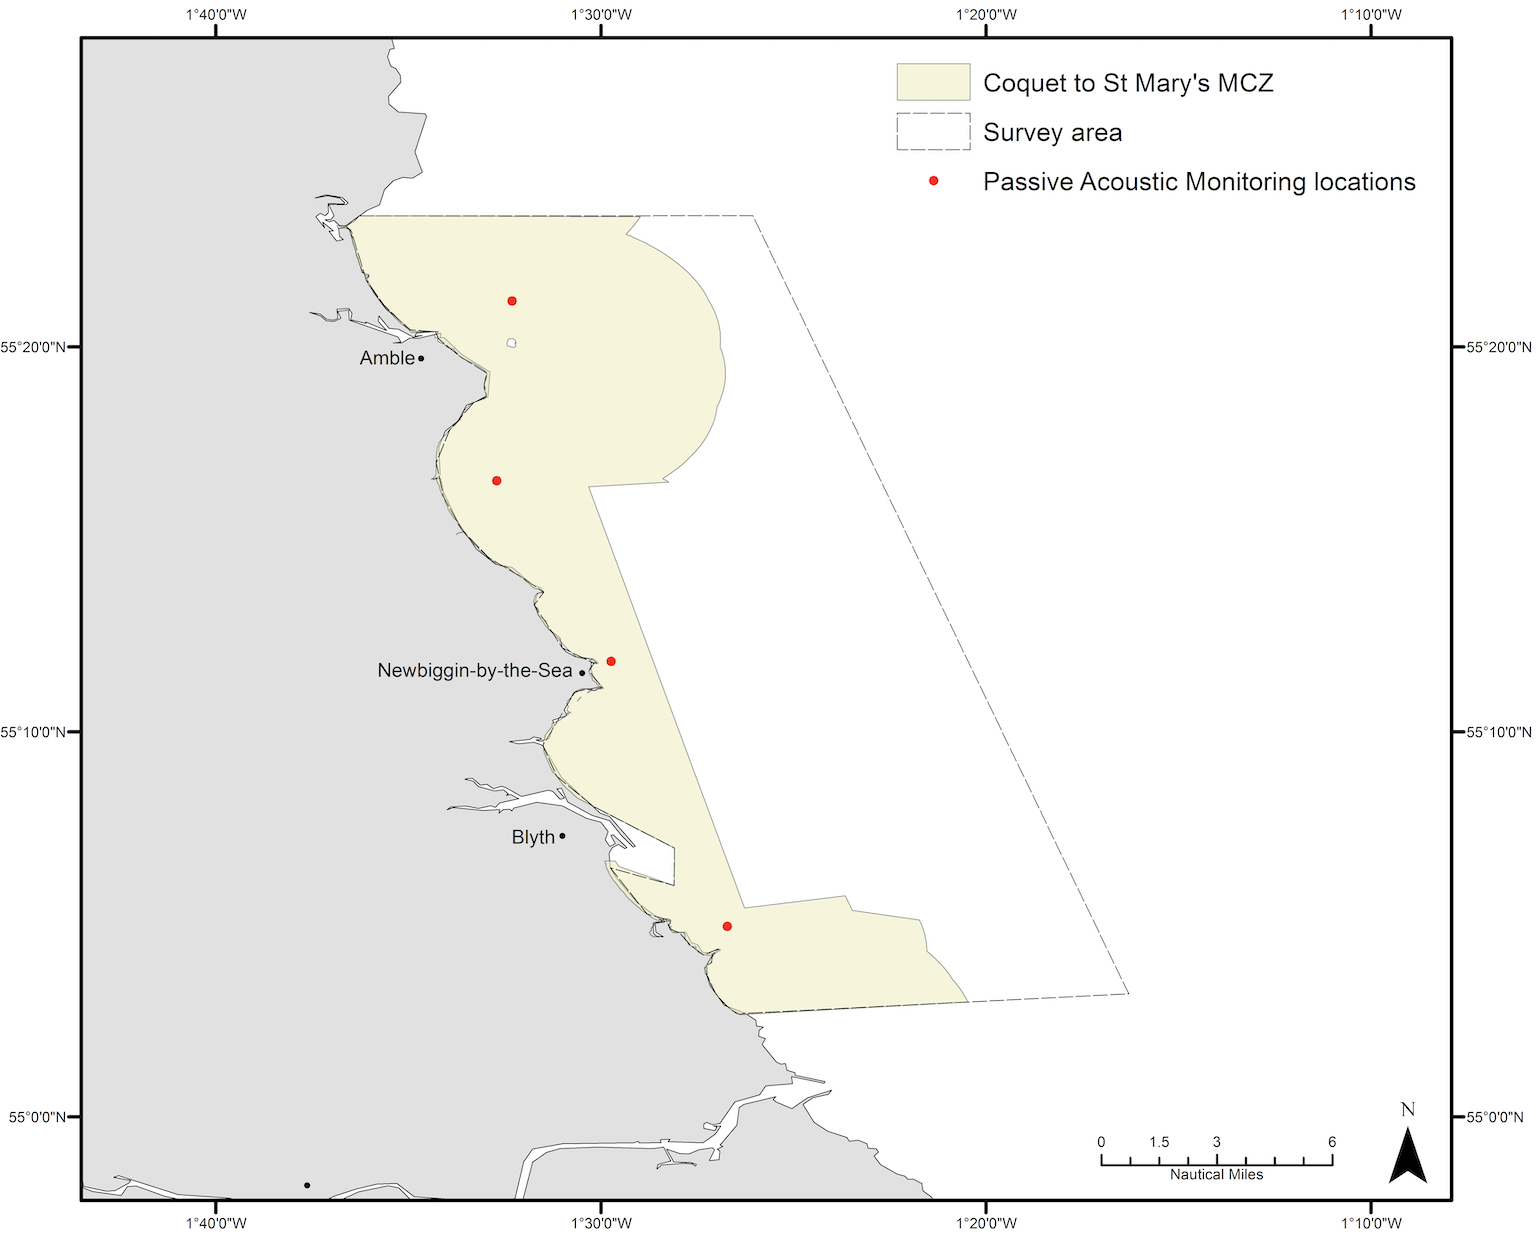
\includegraphics[width=\linewidth]{Chapter1/figs/map.png}
	\end{center}
	\caption{Map of the survey area, Northumberland, UK, from St. Mary's Lighthouse in the south to 25nm above Coquet Island in the north.}
	\label{fig:map}
\end{figure}

With progressively more data being collected during fieldwork through increased use of technology, there is an urgent need for an automatic system for quick identification with reduced error rates. Previous efforts to photo-id individuals from underwater video stills from previous expeditions undertaken by Newcastle University's School of Natural \& Environmental Science's Marine MEGAfauna Lab took around three months from raw video file to be completely catalogued. This project addresses these limitations by applying the methodologies, techniques, and computational power of deep learning to the field of marine biology. Deep learning models, specifically Convolutional Neural Networks (CNNs), will be trained on high-end computer clusters using the Microsoft Azure Cloud\footnote{Microsoft Azure Cloud: \href{http://azure.microsoft.com}{azure.microsoft.com}} prior to field studies using existing data. Once trained, the models can be ran on field deployable computers to perform image analysis in real time from multiple data sources (underwater and above water images, and aerial drone footage). Methodologies incorporating these models are designed to quickly identify individuals, assess health, analyse behaviour and incorporate remote sensing techniques. 

CNNs have for many years now been regarded as the main approach for solving image and computer vision related problems. More recently, the development of deep-layered CNNs and the availability of  high-powered GPUs have provided the perfect platform for solving fine-grained computer vision tasks. This project has developed a system to speed up marine cetacean photo-id using a pipeline of CNNs. Starting with a large high resolution image, this pipeline allows for the detection and identification of cetaceans in the image. This system can greatly aid marine biologists, speeding up the identification process allowing for more time to be spent on developing response strategies and health assessments. 

Data collection for this project focussed on a population of white-beaked dolphins (\textit{Lagenorhynchus albirostris}) off the coast of North-East England (see Figure \ref{fig:map}). Recent research has identified sites where the species is regularly sighted \cite{galatius_lagenorhynchus_2016, hammond_cetacean_2013} and underwater image analysis has shown seasonal and multi-year residency. A health assessment based on underwater image analysis identified high incidence of skin disease and trauma suggesting conservation of this population should be high priority \cite{van_bressem_visual_2018}. The species would also serve as a prime sentinel for monitoring North Sea climatic changes as it shows preference for cold water with North-East UK coastal waters representing the southern limit of its range.

\section{Research Problem}

\section{Contributions}

\section{Thesis Structure}

\section{Related Publications}


%%%%%%%%%%%%%%%%%%%%%%%%%%%%%%%%%%
% All nomenclature here for ease
\nomenclature[z-CNN]{CNN}{Convolutional Neural Networks}
\nomenclature[z-CV]{CV}{Computer Vision}
\nomenclature[z-CPU]{CPU}{Central Processing Unit}
\nomenclature[z-GPU]{GPU}{Graphical Processing Unit}
\nomenclature[z-SGD]{SGD}{Stochastic Gradient Descent}
\nomenclature[z-SGDR]{SGDR}{Stochastic Gradient Descent with Restarts}
\nomenclature[z-ReLU]{ReLU}{Rectified Linear Unit}
\nomenclature[z-FCN]{FCN}{Fully Convolutional Network}
\nomenclature[z-RPN]{RPN}{Region Proposal Network}
\nomenclature[z-VM]{VM}{Virtual Machine}
\nomenclature[z-MCZ]{MCZ}{Marine Conservation Zone}
\nomenclature[z-RIB]{RIB}{Rigid Inflatable Boat}
\nomenclature[z-NDD20]{NDD20}{Northumberland Dolphin Dataset 2020}
\nomenclature[z-SMRU]{SMRU}{Sea Mammal Research Unit}
\nomenclature[z-PCA]{PCA}{Principle Component Analysis}
\chapter{Background}\label{ch:Background}

In recent years, deep learning has become a widely used technique to tackle problems faced in a wide variety of areas. Deep learning models, large neural networks capable of exploiting abstract patterns in data to solve a task, have consistently been shown to outperform other machine learning techniques \cite{lecun_deep_2015, zhang_machine_2017, korotcov_comparison_2017, paterakis_deep_2017}. As an extremely fast paced and every growing field it would not be possible to explore the entirety of deep learning, and as such this Chapter will focus primarily on deep learning in a computer vision context, exploring and understanding image data. 

One novel area where computer vision and deep learning can play an important role is in the world of marine conservation, helping to automate a currently labour intensive discipline. This project focusses on the automation of cetacean photo-identification, a process utilised by conservationists for tasks such as population estimates and health assessments \cite{holmberg_estimating_2009, cheney_long-term_2014, lockyer_observations_1990, van_bressem_visual_2018}. Before research undertaken in this project is discussed, this Chapter will seek to provide an introduction to both photo-identification and deep learning, before expanding into how this has been applied to computer vision. Literature focussing on computer vision in a cetacean conservation space is explored, as well as the current state of fine-grained recognition - utilising computer vision algorithms to differentiate between visually similar classes.

\section{A Brief Introduction to Photo-Identification}\label{ch:Background,sec:photo-id}

One of the main goals of conservation research is to monitor resident animal populations in a given geographic area. This is most commonly performed using mark-recapture surveys in which researchers identify the number of unique individuals in an area at a given time, before returning to the same area at a later point in time and again identifying the number of individuals present \cite{constantine_abundance_2012, bigg_assessment_1982, sharpe_indian_2019}. These values allow for an estimate of the total population size to be obtained, with the accuracy of this value increasing proportionally to the number of surveys undertaken. These mark-recapture surveys can be classified as either invasive, where animals are physically trapped, tagged, and released, or non-invasive where monitoring is performed passively. 

Photo-identification, often abbreviated to photo-id, is one of the main non-invasive mark-recapture methods utilised by cetacean researchers \cite{hammond_individual_1990, evans_monitoring_2004}, usually undertaken over large geographic areas at sea through the use of a small boat although monitoring from coastlines or aircraft may also be utilised \cite{payne_long_1986, forney_seasonal_1998, wursig_methods_1990}. More recently, the use of citizen science has also began to be incorporated within photo-id surveys where evidence exists of smaller species population densities over large areas which may make full-scale monitoring infeasible \cite{gibson_using_2020, cheney_integrating_2013}.

Initially utilised for the tracking of individual distinctive animals within a species \cite{caldwell_evidence_1955, schevill_daily_1960}, the methodology was quickly adapted to large-scale monitoring of whole pods \cite{alves_population_2013, franklin_migratory_2008}. Photo-id has been utilised for the monitoring of multiple cetacean species, with proven use cases on a variety of cetacean species such as Indian Ocean humpback dolphins (\textit{Sousa plumbea}) \cite{sharpe_indian_2019}, Risso's dolphins (\textit{Grampus griseus}) \cite{miragliuolo_rissos_2004}, Northern bottlenose whales (\textit{Hyperoodon ampullatus}) \cite{feyrer_origin_2021}, and killer whales (\textit{Orcinus orca}) \cite{bigg_assessment_1982}. Outside of cetaceans, photo-id has further found use studying other marine life such as whale sharks (\textit{Rhincodon typus}) \cite{holmberg_estimating_2009}, sea turtles (both \textit{Chelonia mydas} and \textit{Eretmochelys imbricata}) \cite{reisser_photographic_2008}, and Florida manatees (\textit{Trichechus manatus latirostris}) \cite{langtimm_survival_2004}. Land based photo-identification studies are also possible, with Goswami \textit{et al.} utilising photographic data to estimate demographic parameters of Asian elephants (\textit{Elephas maximus}) \cite{goswami_application_2007id}.

As can be seen from the examples of species where photo-id is utilised, this methodology for mark-recapture relies on the species having some form of individually identifiable markings, similar to human fingerprints. Typically, this identifying information is located on a part of the body which is likely to breach the water at some point during an encounter - examples of underwater photo-id do exist however the practise is not yet commonplace \cite{vanbressem_visual_2018}. Depending on the species of animal, different parts of the body are the primary identifying location; for dolphins this is usually the dorsal fin whilst for whales this is primarily the fluke, or callosities if present \cite{vernazzani_eastern_2013, arnbom_individual_1987, constantine_abundance_2012, sharpe_indian_2019, baird_population_2009}. See Figure \ref{fig:body-parts} for examples.

\begin{figure}
	\begin{center}
		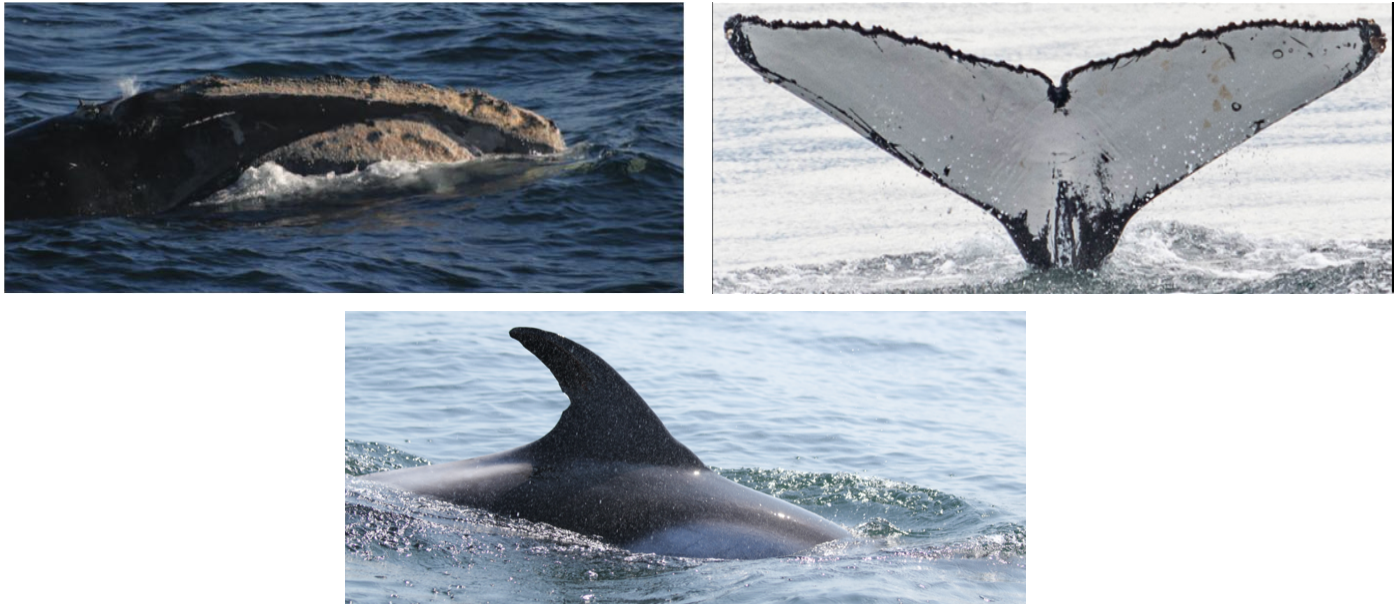
\includegraphics[scale=0.6]{Chapter2/figs/body-part-examples.png}
	\end{center}
	\caption{Examples of the main body parts utilised in cetacean photo-id. Left: callosities present on the head of a northern right whale (\textit{Eubalaena glacialis}) \cite{perrin_encyclopedia_2009}. Right: fluke of a humpback whale (\textit{Megaptera novaeangliae}) \cite{cheeseman_happywhale_2019}. Bottom: dorsal fin of a common bottlenose dolphin (\textit{Tursiops truncatus}) \cite{trotter_ndd20_2020}.
	}
	\label{fig:body-parts}
\end{figure}

During photo-identification surveys, researchers will often focus on long lasting markers such as body-part shape, nicks, notches, and pigmentation which have been shown to be stable throughout the life of the animal \cite{wursig_photographic_1977, lockyer_observations_1990, mann_cetacean_2000}. In some cases secondary markers, those which may heal and are thus not stable such as scarring, may also be utilised for identification. These secondary markers may be anthropogenic, for example from collision with a vessel, or natural, for example from encounters with prey. Scarring is of particular use when identifying Risso's dolphins who are well known for the persistent nature of their scarring, which is thought to occur due to a loss of pigmentation when their scars heal \cite{mariani_analysis_2016}. Pigmentation also occurs in other cetacean species such as striped dolphins (\textit{Stenella coeruleoalba}) and has been used for photo-identification where it can be considered a primary marker \cite{rosso_colour_2008}.

Regardless of the species being analysed or the body-parts used during photo-id it is imperative that the process is standardised, allowing for works to be compared over spatial and temporal scales. This process began in 1988 through workshops held by the International Whaling Commission, with further recommendations published in 2015 by Urian \textit{et al.} \cite{hammond_individual_1990, urian_recommendations_2015}. This standardisation process requires some assumptions to be universally made. For one, all of the markers must be considered stable, that is, they must not fade over the years. Even if a photo-id study only occurs over a few years, the markers utilised must be stable enough so that if another survey is conducted in the same area in later years, individuals from the first study must still be identifiable - providing useful information to health assessments, population estimates, and residency surveys. This stability reduces false negatives, where one individual is recorded as multiple over time. Second, the markers must be considered individually unique. Those chosen to identify an individual must not overlap with other individuals in the survey area. This reduces the chance of false positives, where multiple individuals are recorded as one. Chosen markers must also allow for a consistent re-sighting probability over time. This is critical for abundance estimates,  ensuring that an individual's chosen markers provide it with the same chance of being spotted one year as another. As such, it is extremely important that photo-id methodologies are standardised, both at an international level and between researchers in the same organisations. 

Because of the assumptions which must be adhered to, as well as the manual nature of the photo-id process, there are many downsides. Being able to identify individuals relies on high quality photographs. Thanks to the advent of digital photography and the relative inexpensiveness of cameras capable of capturing large megapixel images, this is less of an issue than before, although it still must be considered. Surveys can also only be undertaken in good weather conditions in terms of sea state and lighting, both of which can affect the chance of an accurate match. These conditions are harder to meet in some areas of the world, reducing the suitability of photo-id for some geographic areas. Conditions, as well as the nature of the animal itself, may make photographing both sides of the individual impossible. Markings are rarely duplicated on both sides of an individual, and thus not having both sides may make matching difficult. For example, an individual may have an extremely distinctive marking on the left side of their dorsal fin however if only the right side of the individual has been captured, when the left side is also eventually photographed it may be labelled as a new individual as no previous examples of the individual's left side exist in the catalogue. If the individual has a very distinct fin shape then this issue can be overcome, although this may not always be possible. As such, individuals may not be added to a catalogue without both sides of the fin available for later comparison. 

Furthermore, photo-id as a whole is extremely labour intensive. Unlike land based camera trap systems, marine based photo-id surveys require a large human effort. Staff are needed not just for photographic purposes, but also for piloting of vessels. As the surveyed animals are free roaming, large spatial areas must be covered, and there is no guarantee of encountering them during a given day. Back on land, the captured photographs must then be manually analysed and the individuals in them identified. This can often take longer than the entire data collection period. Thanks to the labour intensiveness  of the photo-id process, it can also be extremely costly to undertake. Staff need to be paid, vehicles need to be fuelled, and equipment must be maintained. Because of this, any solutions which may speed up the photo-id process would be welcomed both by researchers and their funding bodies. 

\section{Supervised and Unsupervised Learning}\label{ch:Background,sec:DLIntro,sub:supervisedVsUnsupervisedLearning}

Within machine learning as a whole, the vast majority of tasks can be placed into two categories, supervised or unsupervised learning. 

\textbf{Supervised learning} tasks are those where the model can be trained using an input and expected output value pair, known as a ground truth. This technique lends itself well to tasks such as classification, where an input can be mapped to a set of defined output classes, or in regression where an input can be mapped to a continuous output space. 

Training is performed by splitting the available data into training and test sets, with the former being used to train the model and the latter being used to test the model's performance on previously unseen data. Both the training and test set contains ground truth data, but only the training set's influences the generalisation of the model. For example, in the case of a dog or cat classifier a dataset may contain 1000 images, some labelled as \texttt{dog} and some as \texttt{cat} (the ground truths). This data will then be split randomly into a training and test set; for example 80\% of the data used for training with 20\% used for testing. The classifier will then iterate through the training set, using the ground truth values to train the network's parameters in a way to best generalise the model. After training has been completed the model will then be evaluated against the test set. Each data point will be processed by the model and a prediction outputted, which is then compared to the unseen ground truth to provide an evaluation of the model's performance.

\textbf{Unsupervised learning} tasks are, in contrast, those where prior ground truths for your data are not available. This approach lends itself well to clustering and aiding in understanding of the underlying data structure. These unsupervised algorithms, such as K-Means clustering \cite{hartigan_algorithm_1979}, are not provided guidance on how to group the data given, but are rather left to discover interesting structure on their own. 

Taking the dog and cat data again as an example, it is clear how this data could be clustered in an unsupervised manner. Asking the clustering algorithm to provide two clusters for the data  (e.g. $K = 2$), a model could be trained to split the data with all dogs in one cluster and all cats in the other, without having to be told which images are dogs and which are cats. However due to the unsupervised nature of the learning process, the model is equally as likely to cluster the data based on whether the animal is, for example, sitting or standing. 

\section{A Brief Introduction to Deep Learning}\label{ch:Background,sec:DLIntro}

Deep learning aims to create artificial networks to complete tasks through a learning process, in a similar way to how neurons in the human brain operate. These computational models are made up of neurons and are often multiple layers deep. Lower layers represent basic abstractions building up from this as you go \textit{deeper} into the network. Layers at the deepest points can, based on information passed to them from lower levels, begin to provide estimations of answers to a given problem. In literature neural networks are often illustrated in forms similar to Figure \ref{fig:NN-example}, which shows a visual representation of the VGG16 architecture \cite{simonyan_very_2015}. 

\begin{figure}
	\begin{center}
		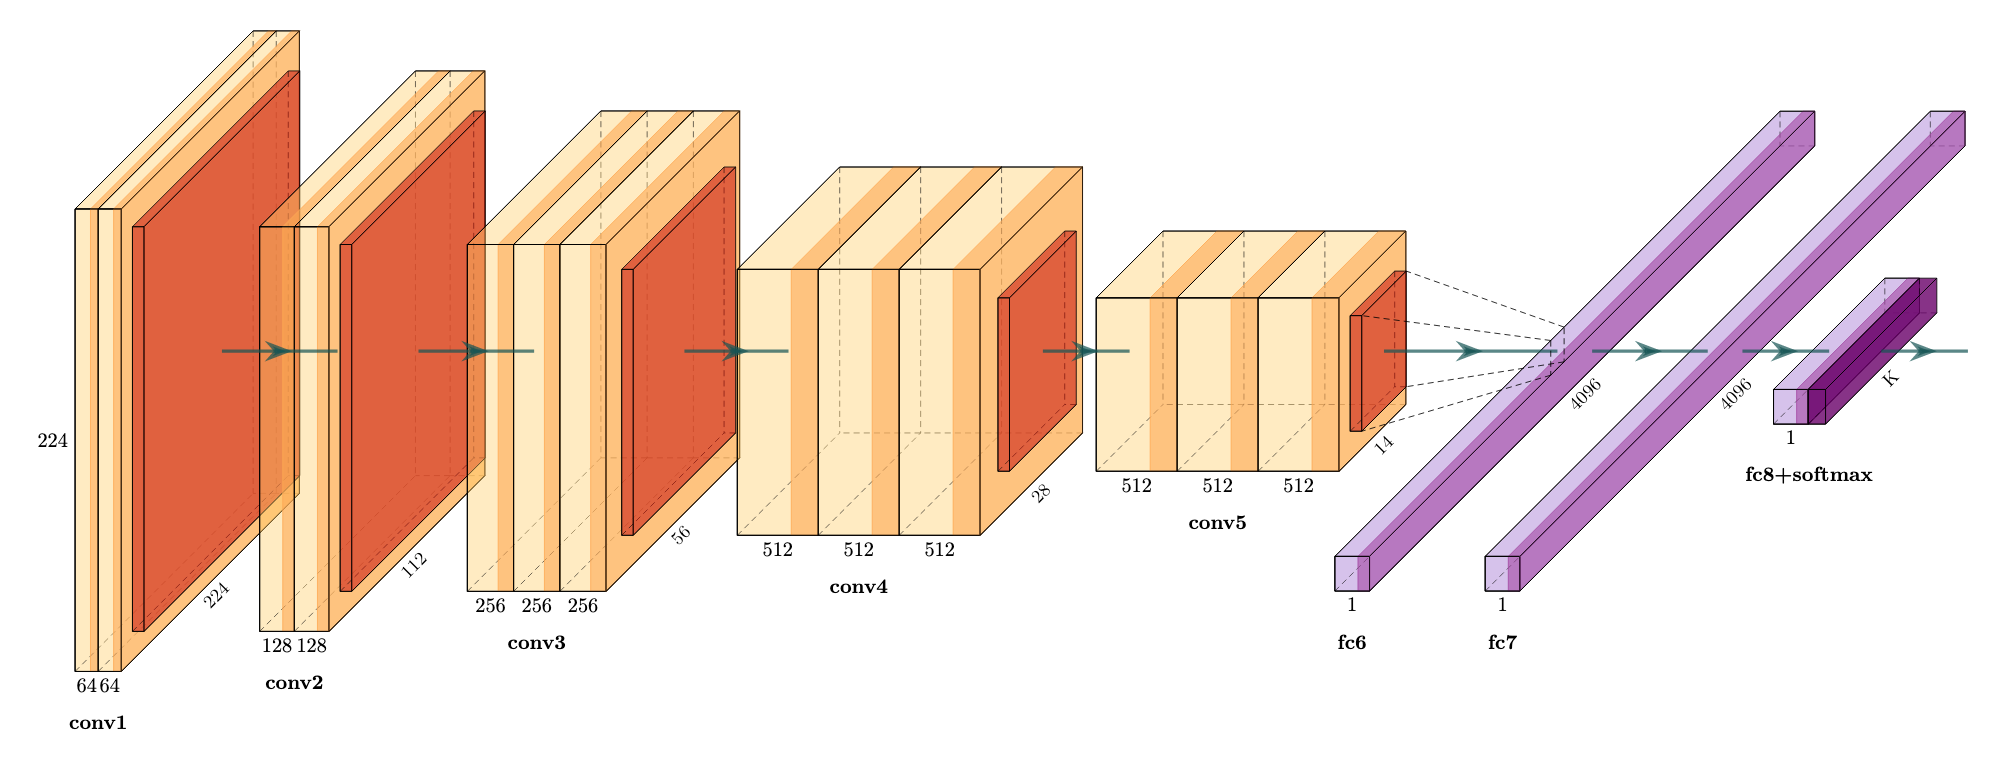
\includegraphics[scale=0.2]{Chapter2/figs/example-model.png}
	\end{center}
	\caption{An example neural network architecture diagram, showing VGG16 \cite{simonyan_very_2015}. Data is inputted to the network at the leftmost layer before being passed through the layers sequentially. The rightmost layer provides the overall output of the network, such as a classification or probability. \cite{harislqbal88_plotneuralnet_2018}}
	\label{fig:NN-example}
\end{figure}

This ability to learn directly from the data provided is the key difference between deep learning and more classical machine learning techniques, which often require considerable domain expertise to design a feature extractor allowing for raw data values, such as pixels, to be transformed into a feature vector suitable for a model to learn. This can be seen as deep learning democratising machine learning thanks to the model learning purely from the data rather than any bias added in by humans which may be present using non-deep learning approaches.

Deep learning models in contrast are capable of learning to performing tasks such as classification on raw data values through multiple layers of simple non-linear transformations. For example in the case of computer vision, lower layers of neurons are optimised by the network itself to learn lines and basic shapes, middle layers may be optimised to learn more complex ideas such as how these lines and shapes fit together, with the final layers providing an output of object label (e.g. \texttt{dolphin}). It should be stressed however that the features these layers are looking for are not specified by humans, but rather learned from the data by updating their parameters predominantly through optimisations such as stochastic gradient descent and backpropagation \cite{hecht-nielsen_iii.3_1992}.

This ambition to create artificial networks similar to how the brain operates stems mainly from work undertaken in 1943 by McCulloch and Pitts \cite{mcculloch_logical_1943} in an attempt to understand how neurons in the brain allow for the understanding of complex patters. This model formed the basis of future work into machine learning, and thus deep learning. This work continued at small scale for many years. It has only been recently thanks to advances in availability of large scale datasets needed to train these networks and power of the computing resources available has deep learning research accelerated. The transition to training on clusters of high-powered GPUs has allowed for a significant speed-up in both model training and inference time compared to traditional CPUs, allowing for a higher amount of prototyping in a smaller time frame \cite{luo_artificial_2005}. Further to this, the advent of cloud computing has allowed for much more cost-effective model development. Thanks to the Pay As You Go model of computing now commonplace cloud providers have reduced the need for researchers to acquire their own hardware for model training - although many argue it is still cheaper to buy your own in the long term. 

More so, advances in deep learning have been helped greatly through the development of standard development frameworks. Google's Tensorflow \cite{abadi_tensorflow:_2016} and Facebook's PyTorch \cite{paszke_automatic_2017} allow for researchers to develop models much faster than previously due to their reduction in the amount of boiler-plate code needed, with these frameworks often doing a lot of the \textit{heavy lifting} in the background. Further advances have been made through the availability of large scale coarse-grained datasets such as MNIST \cite{lecun_gradient-based_1998}, Caltech-256 \cite{griffin_caltech-256_2007}, and ImageNet \cite{deng_imagenet:_2009} allowing for common baselines to be adopted by the computer vision community and for the introduction of transfer learning, allowing for the reuse of models trained in one task to be utilised for another \cite{pan_survey_2010}. Furthermore, additional regularisation techniques have provided improvements to model accuracy. Notable examples of this in literature which are now commonplace in deep learning models include dropout \cite{srivastava_dropout:_2014}, batch normalisation \cite{ioffe_batch_2015}, stochastic gradient descent with warm restarts \cite{loshchilov_sgdr:_2016}, and mixup \cite{zhang_mixup:_2017}. The use of data augmentation is also commonplace. This is where existing data will be perturbed randomly to create new, artificial data. Examples of image data augmentation include simple perturbations such as random horizontal and vertical flipping, and cropping, as well as more complicated techniques like Gaussian blurring, perspective shifting, and colour jitter.

\subsection{Optimising the Deep Learning Network}\label{ch:Background,sec:DLIntro,sub:stochasticgradientdescent}

In order to generalise our deep learning models, we need to be able to optimise the parameters within each individual neuron. These parameters can either be weights which control the strength of the connection between two neurons, or biases - a constant additional input which guarantees a neuron's value can never be zero. Most commonly, this is performed using gradient descent to minimise a loss function (a measure of distance between ground truth and prediction). If this function were to be visualised on a graph each parameter would be represented by an axes, resulting in a hyper-surface with millions of dimensions in the case of deep learning models. The goal of network optimisation is to find the minimum point on the hyper-surface, as this would give the parameter values which produce the smallest loss. Loss functions however are non-convex \cite{choromanska_loss_2015}, which can result in multiple local minimums. In order to find the (hopefully global) minimum point on the hyper-surface, during training the model's weights must be updated iteratively in the \textit{opposite} direction of the gradient of the loss function's hyper-surface. As such, we follow the direction of the slope of the hyper-surface downhill until we reach a minima, an area where the loss is lowest \cite{ruder_overview_2016}. Before the advent of deep learning and big data, it was common for the whole dataset to be used to compute the gradient at each iteration; however due to the size of modern day datasets this is no longer possible due to the computational cost this would impose on the system. As such batches, a small random subset of the larger dataset, are often used to give an estimation of the overall loss gradient.

In order to reach this minimum, a process known as stochastic gradient descent (SGD) is most commonly used. At each iteration of SGD, a batch will only contain one randomly selected training example. The loss for this example is calculated, and used to step down the gradient slope, rather than the sum of the loss' gradient over all training examples. As we only take one example per iteration, the path taken down the slope to the minima is far noisier and random than the path obtained from using all examples, hence the \textit{stochastic} nature of the gradient descent. This stochastic nature does result in a longer convergence time to the minima compared to non-batch gradient descent, however this is outweighed by the reduction in computational expense. The use of SGD often leads to a good set of model weights quickly compared to other, more elaborate techniques \cite{bottou_tradeoffs_2008}. 

In recent years there have been efforts to modify SGD in an attempt to improve model optimisation. The most commonly seen optimisations within production code include SGD with warm restarts (SGDR) \cite{loshchilov_sgdr:_2016}, Momentum \cite{qian_momentum_1999}, RMSProp \cite{tieleman_lecture_2012}, Adam \cite{kingma_adam:_2014}, and AMSGrad \cite{reddi_convergence_2019}. Work in this thesis utilises SGDR and Adam primarily. All of these optimisations attempt to stop the problem of getting stuck in local minima rather than the global minimum of the overall loss function. However, recent studies show that the problem of local minima is not as big as first thought and, regardless of initial conditions, vanilla SGD rarely gets stuck in local minima \cite{dauphin_identifying_2014, choromanska_loss_2015}.

\subsection{Backpropagation}\label{ch:Background,sec:DLIntro,sub:backprop}
As discussed in Section \ref{ch:Background,sec:DLIntro,sub:stochasticgradientdescent}, we have seen how weights and biases in each neuron can be learnt and optimised using SGD. However, it is important that we also discuss how the gradient is computed. This computation can be performed relatively quickly using backpropagation, or the backward propagation of errors algorithm. Before delving \textit{too deep} into deep learning, it is of imperative importance to understand backpropagation; it is after all often cited as one of the cornerstones of deep learning \cite{alber_backprop_2018}.

Backpropagation was originally described in Linnainmaa's masters thesis from 1970 \cite{linnainmaa_representation_1970}, although its effect was not fully realised until 1986, when Rumelhart \textit{et al.} discussed the advantages to using backpropagation over other learning approaches \cite{rumelhart_learning_1986}. In recent years multiple works have provided updates and improvements to the original backpropagation algorithm, however none have seen wide-scale adoption \cite{bengio_use_1994, lillicrap_random_2014, lee_difference_2015, nokland_direct_2016, liao_how_2016}. 

The standard backpropagation algorithm to compute the gradient of the loss function w.r.t a model's layers is, in essence, the chain rule (a formula for computing the derivative of multiple functions). Working backwards through the network, the last layer's gradient is first calculated providing a partial calculation of the overall network's gradient. This is then used to efficiently calculate the layer above's gradient, propagating information regarding the loss and how weights should be changed throughout the network. This backwards propagation is a far more computationally efficient way of calculating the overall loss gradient compared to calculating each layer's gradient loss in isolation. Further efficiencies have been made thanks to deep learning frameworks implementing backpropagation in a way that takes advantage of GPUs, leading to extremely efficient computations when performing deep learning tasks such as object detection and other computer vision tasks.


\section{Deep Learning for Computer Vision}\label{ch:Background,sec:DLforCV}

The field of computer vision, allowing computers to gain and interpret knowledge from image and video data, is one area where deep learning has excelled \cite{voulodimos_deep_2018}. Generalisable concepts such as Convolutional Neural Networks (CNNs) have quickly become commonplace for solving computer vision tasks, in most cases replacing the need for hand-crafted pipelines specialised to the task at hand, thanks to their ability to learn complex patterns in data where there is a strong spatial and temporal dependency between the values. This ability is essential for processing image data which is, at it's most basic level, a matrix of pixel values. These matrices are three dimensional, representing an image's height, width, and depth, where depth is dependant on the colour model used to represent the image. The most common of these models is RGB which has channels representing the red, green, and blue colour present in an image; as such a matrix representing an RGB image will have a depth of three. Other colour models have varying depth values, a greyscale image would have a depth of one for example, whilst a CMYK image which have cyan, magenta, yellow, and black colour channels would have a depth of four. As can be imagined, these matrices can very quickly reach unworkable sizes. An RGB image at 1080p resolution for example would require a matrix of size 1920x1080x3, or 6,220,800 values. CNNs utilise a set of standard operations which are capable of reducing image sizes down to a more workable form whilst still retaining key features which all for inference to occur. 

\subsection{Convolutional Neural Networks}\label{ch:Background,sec:CNN,sub:CNN}
Modern CNNs are composed of three main layer types; convolutional layers, pooling layers, and fully connected layers. Each of these layers will perform some operation on the input matrix passed to it, and provide a transformed output to the subsequent layer(s). These layers can be stacked in various orientations to build different CNN architectures.

\subsubsection{Convolutional Layers}\label{ch:Background,sec:CNN,sub:CNN,subsub:convolution}

The convolutional layer is the workhorse of the CNN, performing the vast majority of the operations required. Convolutional layers utilise what is known as a kernel in order to efficiently extract features from an input image matrix. A kernel is a matrix, most commonly 3x3 or 5x5 in size, which represents some weighting refined through training. This kernel is slid over the input data computing the dot product between the weights and the section of the input matrix it is currently over, before summing these into a single value. This gives an output matrix of features represented by the weighted sum of the input, known as a feature map. These feature maps generally represent basic shapes at shallow levels, which are then built on as the model gets deeper, representing more complex shapes as you progress. A visual representation of how convolution is performed can be seen in Figure \ref{fig:kernels}.

The kernel process can be performed multiple times over the same input using different weightings, giving multiple output feature maps. In the case where there are multiple input dimensions (such as an RGB image), kernels are required to operate over all dimensions. As such, the resulting feature maps are summed element-wise, along with some bias term, to produce a single output map. 

The size of the kernel as such determines the number of input features which are combined to give the new output feature map, although the size of the resulting map is determined also by two other properties; stride and padding. Stride refers to the distance in pixels the kernel will move when performing the next input mapping. For example, a stride of 1 would result in the kernel sliding along one pixel value each time, resulting in an output feature map of equal size to the input, whereas a stride of 2 would skip every other pixel, reducing the output feature map by half. 

A problem can arise during convolution when the kernel reaches the edges of the input matrix. As there is nothing past the edge values, these values must be trimmed as they are never in the centre of the kernel. This can cause the reduction of the matrix, as some values are never utilised, which may be detrimental when we require an output feature map which is the same size as that of the input. As such, padding can be performed. This technique places zeros around the edges of the input matrix, expanding it's size and allowing pixel values formerly at the edges to be utilised by the kernel. 

\begin{figure}
	\begin{center}
		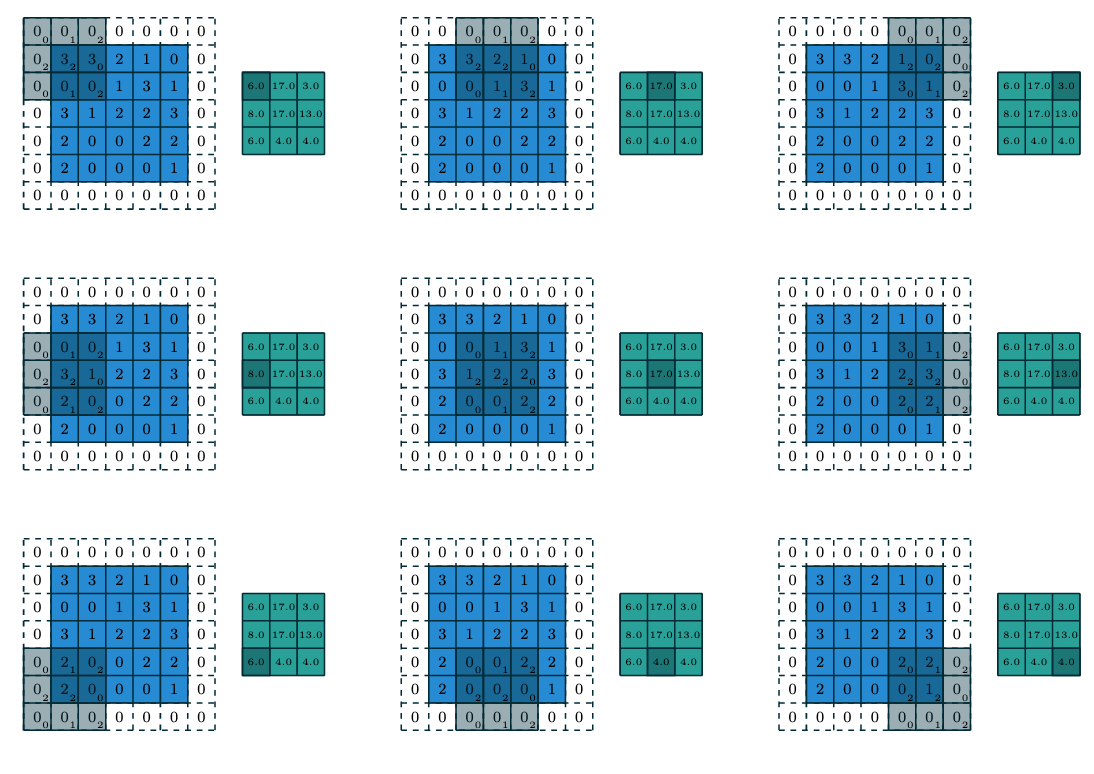
\includegraphics[scale=0.45]{Chapter2/figs/kernel.png}
	\end{center}
	\caption{A visual representation of convolution. A kernel, represented by the grey squares, operates over a padded input matrix, blue, with a stride of 2 to produce an output feature map, green. Note that the kernel's weights are denoted by the number in the lower right of each box and the input pixel value is denoted by the number in the middle of each box. Image from \cite{dumoulin_160307285_2018}}.
	\label{fig:kernels}
\end{figure}


\subsubsection{Pooling Layers}\label{ch:Background,sec:CNN,sub:CNN,subsubsec:pooling}

Pooling layers help reduce the computational complexity of the convolutions performed by the CNN. This is achieved by reducing the spatial dimensions of the input ready for the next convolutional layer through the use of some function applied over batches of the input pixel values, similar to how a kernel operates in a convolution layer by sliding over the image. Pooling only affects the width and height of the input, not the depth, as all depth channels are required to keep the colour mapping of the image intact. 

Pooling as such inevitably leads to a reduction in the amount of information available to subsequent layers; this is advantageous however as it leads to less computational complexity, aiding in the minimisation of overfitting in the model. 

A number of different pooling layer architectures exist in literature, such as max pooling which only keeps the maximum pixel value in the batch, average pooling \cite{boureau_theoretical_2010} which outputs the mean of all pixel values in the batch, and stochastic pooling \cite{zeiler_stochastic_2013} which selects an output pixel value from each batch based on a probability distribution. For a review of current pooling methods, see \cite{gholamalinezhad_pooling_2020}.

\subsubsection{Fully Connected Layers}\label{ch:Background,sec:CNN,sub:CNN,subsubsec:fullyConnected}

Fully connected layers take feature maps produced by the preceding convolutional and pooling layers and reduce these down to a single $N$-dimensional vector, where $N$ represents the total number of classes and each dimension's value is the probability of the class. These probabilities are achieved using a softmax activation function. The activation function is responsible for deciding which neuron in the layer passes it's value to the layer below by computing the weighted sum of the inputs and passing the result through a non-linear function. Softmax takes the exponents of each input and normalises them by the sum of all inputs, giving values between 0 and 1. Outputted $N$-dimensional vectors can then be considered a feature map in their own right for further processing \cite{krizhevsky_imagenet_2012} or as a category for classification as the last layer of the network \cite{girshick_rich_2014}.

\begin{figure}[!hb]
	\begin{center}
		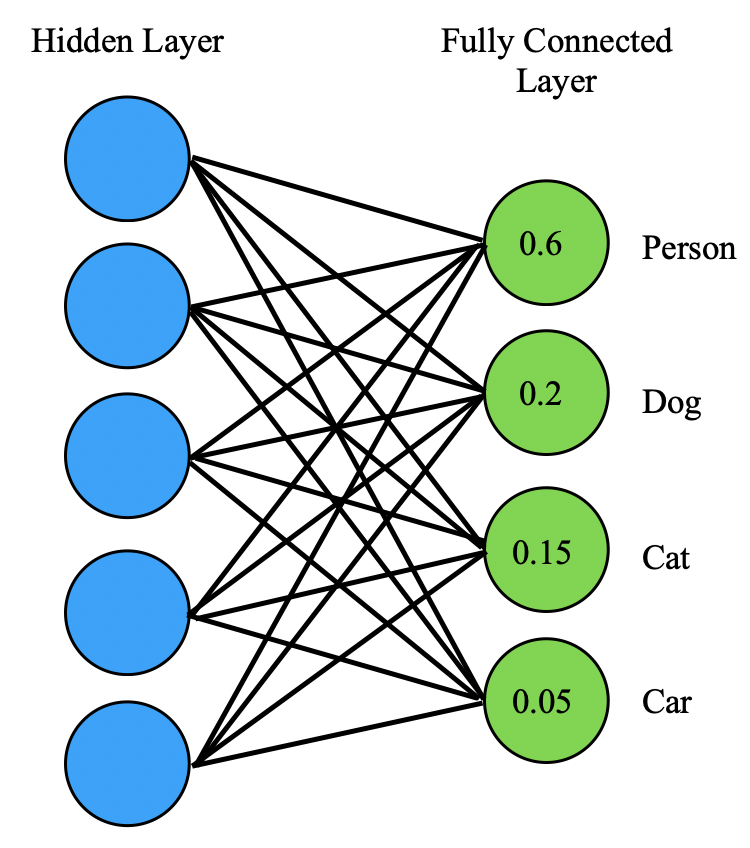
\includegraphics[scale=0.45]{Chapter2/figs/fully-connected.png}
	\end{center}
	\caption{A visual representation of the final stages of a classification network. The leftmost blue circles represent the final hidden layer in the network, with the rightmost green circles representing the fully connected layer. Each neuron in the hidden layer is connected to all neurons in the fully connected layer. The value in the hidden layer's neurons represents the activations after softmaxing, with the label denoting the class represented by the neuron. The network has predicted the input to be of class \texttt{Person}.}
	\label{fig:fully-connected}
\end{figure}

For example let's assume we have a network who's aim is to classify an image into one of four classes, as seen in Figure \ref{fig:fully-connected}. At the end of this network is a fully connected layer which takes a feature map from the proceeding hidden layer, and produces as output four values between 0 and 1. Each of these values is required to be outputted by its own neuron, resulting in a fully connected layer with four neurons where each neuron represents a possible class for the input image. The image's classification is provided by whichever neuron outputs the highest value. 

\subsubsection{Layer Architectures}\label{ch:Background,sec:CNN,sub:CNN,subsub:layerArchitecture}

Using the three layer types described above it is possible to create an infinite number of CNN architectures. There is no guarantee that every possible architecture will perform well however (indeed, one possible combination would be a single fully connected layer, which would not perform well at all). Whilst it may be advantageous for certain areas of research to create their own custom CNN architecture, either through trial and error or the more recent approach of Neural Architecture Search \cite{elsken_neural_2018}, this is not applicable for most cases. For the vast majority of cases, there exists in literature well-defined generalised CNN architectures, and it is often these architectures which are utilised for computer vision tasks. 

LeNet \cite{lecun_gradient-based_1998} was the first well defined CNN architecture. LeNet was only 7 layers deep, but performed well enough to be applied by some banks for automatic recognition of numbers on cheques. It wasn't until around 2012 that more attention was paid to these defined architectures however, thanks to AlexNet \cite{krizhevsky_imagenet_2012}. Utilising a similar but deeper architecture to LeNet, with more filters and a larger number of stacked convolutional layers, AlexNet also included now commonplace deep learning building blocks such as dropout \cite{srivastava_dropout:_2014}, max pooling \cite{boureau_theoretical_2010}, and ReLU activation functions; the most popular non-linear activation function currently in deep learning, especially in computer vision \cite{he_delving_2015}. ReLU's non-linear function returns 0 for any negative value, or for any positive value $x$, it returns $x$. This can be written as $f(x) = max(0,x)$, and visualised in Figure \ref{fig:relu}. It is this non-linearity that allows for backpropagation to occur.

\begin{figure}
	\begin{center}
		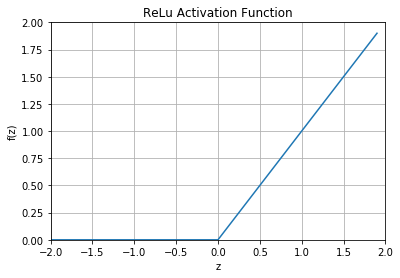
\includegraphics[scale=0.6]{Chapter2/figs/relu.png}
	\end{center}
	\caption{A visualisation of the ReLU Activation Function.}
	\label{fig:relu}
\end{figure}

 In 2014, Google introduced GoogleNet, also known as an Inception architecture, to the ILSVRC14 competition \cite{szegedy_going_2015}. This net achieved a top-5 error rate of 6.67\%, very close to what untrained humans could achieve on the competition dataset, ImageNet \cite{krizhevsky_imagenet_2012}. This was achieved through a 22 layer deep CNN utilising several small convolutions, reducing the number of parameters from 60million in AlexNet to 4million in GoogleNet. 

Finally ResNet was introduced a year later at ILSVRC15. This architecture can be up to 152 layers deep, and achieved a human-beating top-5 error rate of 3.57\% \cite{he_deep_2015}. Shallower versions of ResNet exist, such as ResNet50 and ResNet101, which are 50 and 101 layers deep respectively. This thesis makes use of ResNet50.

\subsection{Object Detection}\label{ch:Background,sec:objectDetection}

Thanks to advancements in deep learning technology and the creation of standardised architectures, CNNs are now utilised en masse to perform tasks such as object detection, attempting to identify distinct regions containing task-specific classified objects in images and video. Whilst this is often performed in one of two ways, it is important to note that all object detection is still in essence a series of tasks performed via network layers. 

\subsubsection{Region Proposal Networks}\label{ch:Background,sec:objectDetection,sub:RPN}

The first, known as a Region Proposal Network (RPN), attempts to find image regions likely to contain objects of given classes. Training data is usually provided in the form of bounding boxes drawn around objects of interest and labelled with the corresponding class. One of the most common and widely used RPN architectures is derived from R-CNN, or Regions with CNN features, architecture \cite{girshick_rich_2014}. R-CNN utilises a selection search \cite{uijlings_selective_2013} to generate 2000 Regions of Interest (RoIs) representing the most likely areas of the input image to contain a class example. By limiting the number of RoIs generated this allows for fast computation compared to operating on every possible region in the image. The proposed RoIs are then fed through a CNN to be classified. See Figure \ref{fig:r-cnn} for a visual representation of the R-CNN pipeline. Example proposed RoIs can be seen in Figure \ref{fig:rpn-randoms}.

\begin{figure}
	\begin{center}
		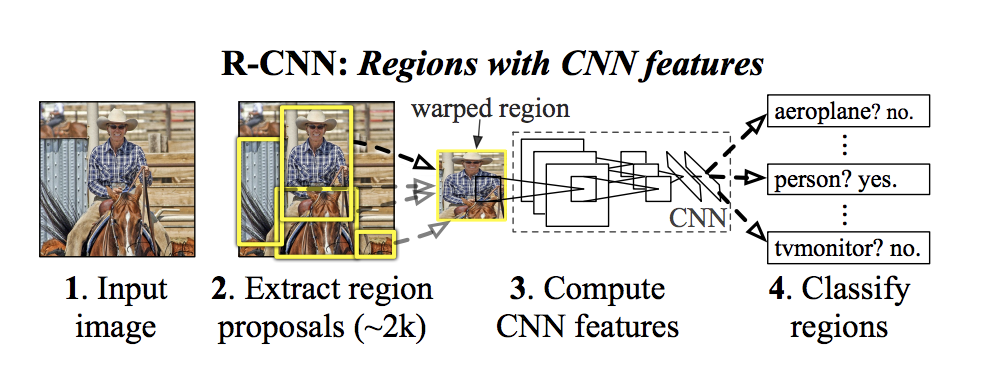
\includegraphics[scale=0.4]{Chapter2/figs/r-cnn.png}
	\end{center}
	\caption{The R-CNN pipeline. Image from \cite{girshick_rich_2014}.}
	\label{fig:r-cnn}
\end{figure}

\begin{figure}
	\begin{center}
		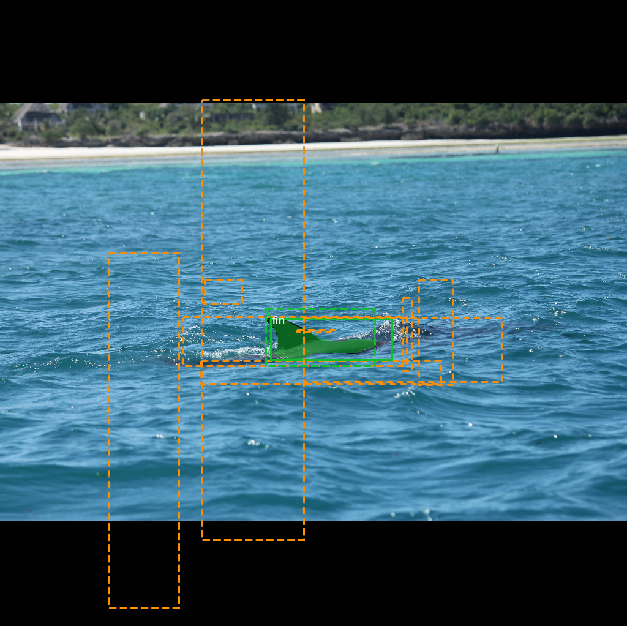
\includegraphics[scale=0.45]{Chapter2/figs/rpn-ten-random-orange.png}
	\end{center}
	\caption{An example of RoIs generated on an image by an RPN, showing 10 random proposals. Note that two of the RoIs have been successfully classified as \texttt{fin}.}
	\label{fig:rpn-randoms}
\end{figure}

Utilising selection search leads to a high recall rate thanks to the large amount of proposals, as there is a high probability that some of these proposals will contain Regions of Interest (RoIs) containing the objects being searched for. However, this can be time consuming and computationally expensive (although less computationally expensive than just sliding a window over the full image) as the network needs to classify the 2000 region proposals generated. Detection can also be slow using an R-CNN and, with the selection search being fixed, no adaptive learning takes place here which may lead to bad region proposal generation. 

Some of these time drawbacks were fixed in later versions of R-CNN, known as Fast-RCNN \cite{girshick_fast_2015}. Rather than feeding the region proposals generated to the CNN, this algorithm instead feeds the input image to the CNN and generates a convolutional feature map. RoIs can then be taken from the feature map using selection search and warped into a shape suitable for the pooling layer, before being reshaped again into a fixed size for the fully connected layer. This is advantageous as it allows us to reuse some computations and allows for backpropagation to occur throughout the network, greatly improving run times.  This also means however that the runtime is dominated by how fast RoIs can be generated. 

To fix this issue, Faster R-CNN was developed \cite{ren_faster_2015}. Now, instead of utilising selection search to generate the RoIs we can utilise a separate network to predict RoIs which can then be used to classify images within the regions. With this, we now train with four losses: 

\begin{enumerate*}
	\item An object/not object classification from the RPN,
	\item The RoI shift,
	\item The object classification,
	\item Final bounding box co-ordinates.
\end{enumerate*}

\subsubsection{Detection Without Proposals}\label{ch:Background,sec:objectDetection,sub:noProposals}

One issue with all RPNs is that they generally take a significant amount of time in order to classify objects in images, with the bottleneck being the region proposal generation. Because of this, there are algorithms which attempt to remove the region proposals altogether and instead look at the whole image. This input image is divided into an equal size grid. Within each square of the grid, we take a set number of bounding boxes which the CNN provides classification confidences for. Any above a set threshold are used to locate the object within the image. These algorithms are essentially one large CNN rather than splitting into a CNN and an RPN and are thus much faster although are not as accurate, especially on smaller objects due to the spatial constraints of the algorithm. Examples of detection without proposal systems include YOLO \cite{redmon_you_2016} and SSD \cite{liu_ssd:_2016}. 

\subsection{Semantic Segmentation}\label{ch:Background,sec:semanticSegmentation}

Along with object detection, semantic segmentation is one of the key research areas in computer vision. Rather than provide RoI bounding boxes as output, semantic segmenters instead output a class label for each pixel in the image. A group of connected pixels of the same class is known as a mask. An example of an image and its masks can be seen in Figure \ref{fig:masks-example}.

\begin{figure}
	\begin{center}
		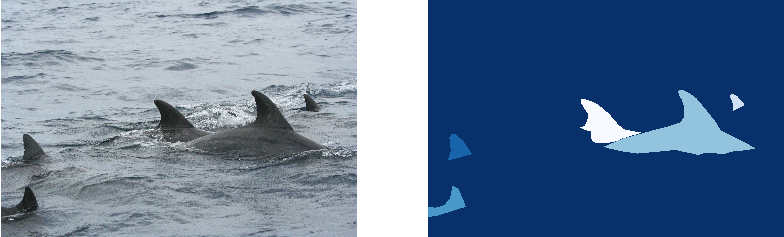
\includegraphics[scale=0.5]{Chapter2/figs/masks-example.png}
	\end{center}
	\caption{An example of an image and its corresponding ground truth \texttt{fin} masks.}
	\label{fig:masks-example}
\end{figure}

In general, semantic segmenters can be thought of as having two main components; an encoder, usually a pretrained classifier built with a standard detection architecture such as ResNet, and a decoder whose job is to project the coarse grain features learnt by the encoder to a fine-grain pixel space. There are two main ways to approach this decoding step.

The first is to use an RPN to perform region based semantic segmentation, extracting the regions from an image and then describing them. Each pixel of the image is then given a classification based on which highest scoring region it is contained in. Note that any pixels not in a region are given the class label of \texttt{background}. This is achieved through the use of a lightweight binary classifier operating over multiple proposal boxes, known as anchors, covering the image at different scales. Each anchor is given an object score denoted by Intersection Over Union (IOU), a measure of how much overlap there is between a model's predicted bounding box and the ground truth. This is taken at a set confidence threshold, usually 50\%, as the model will predict potentially hundreds of boxes for an image, all with different confidence levels. The vast majority of these predictions will be wrong, but will also (hopefully) have very low confidence scores and so they can be safely ignored and thus not counted in evaluation metrics. Taking a predicted bounding box $B_p$ and a ground truth box $B_g$, the IOU between the two can be defined as:

\begin{equation}
IOU = \frac{\text{Area of overlap}(B_p, B_g)}{\text{Area of union}(B_p, B_g)}.
\end{equation}

Anchors with an $IOU >= 0.7$ with any ground truth are donated as positive anchors and are passed on for classification. Those with an $IOU < 0.3$ are considered negative anchors, and those where $0.3 <= IOU < 0.7$ are denoted as neutral anchors and are not used for training. An example of generated negative, neutral, and positive anchors for an image can be seen in Figure \ref{fig:anchor-types}.

\begin{figure}
	\begin{center}
		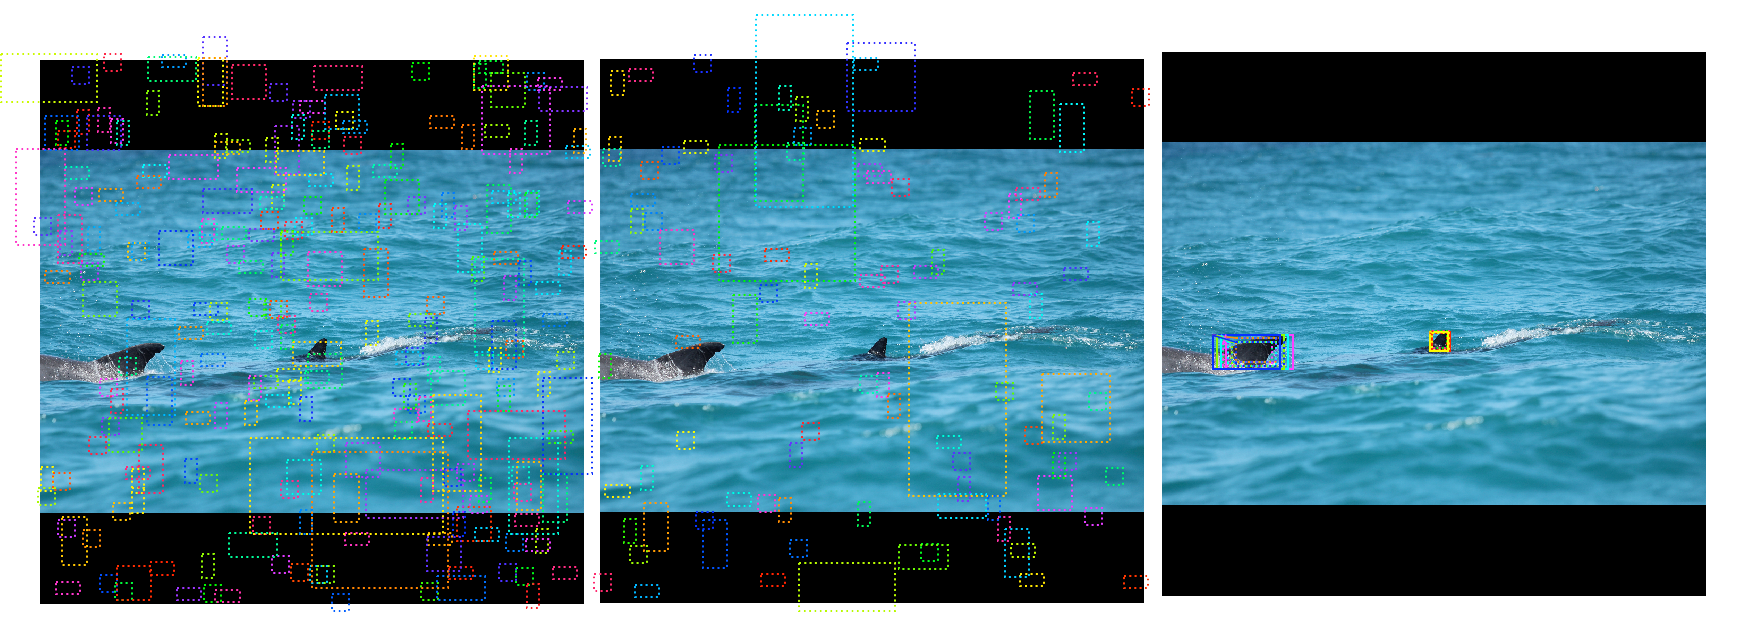
\includegraphics[scale=0.25]{Chapter2/figs/anchor-types.png}
	\end{center}
	\caption{Generated anchors. Left: negative anchors. Middle: neutral anchors. Right: positive anchors.}
	\label{fig:anchor-types}
\end{figure}

In some cases, positive anchors may not fully cover the ground truth object. Because of this, the RPN regresses a refinement applied to the anchors, shifting and resizing them to correct their encasement of the ground truth object. An example of this can be seen in Figure \ref{fig:rpn-refined}.

\begin{figure}
	\begin{center}
		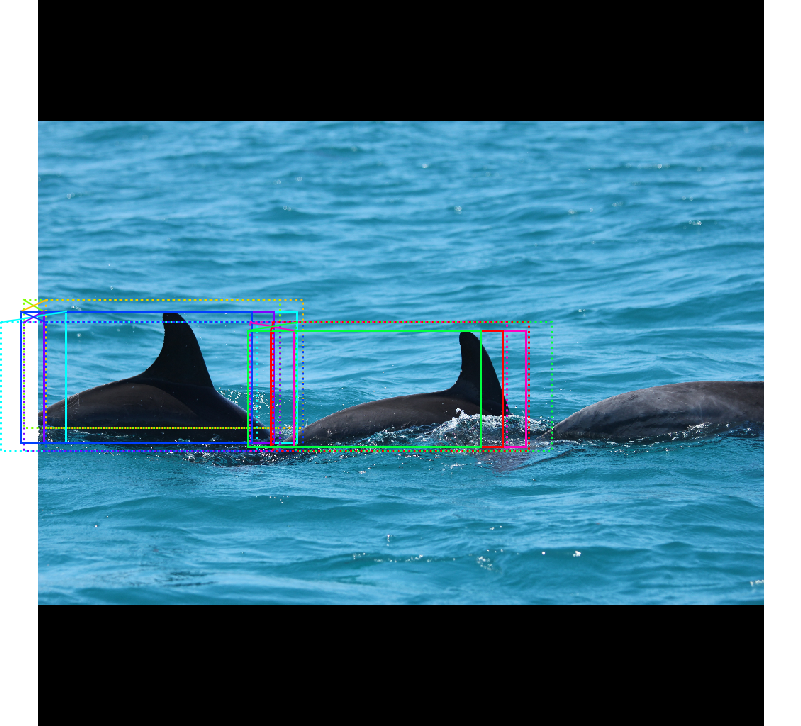
\includegraphics[scale=0.3]{Chapter2/figs/rpn-refined.png}
	\end{center}
	\caption{An example of refined anchors. Positive anchors before refinement are dotted, after refinement are solid.}
	\label{fig:rpn-refined}
\end{figure}

Utilising RPNs does have disadvantages however. Generating the segmentations from the regions take a significant amount of time, and the features generated by RPNs generally do not contain enough feature information to generate well defined masks. Recent research has attempted to fix these issues, such as SDS \cite{hariharan_simultaneous_2014} or Facebook's Mask R-CNN \cite{he_mask_2017}. This thesis makes use of Mask-RCNN.

Fully Convolutional Networks (FCN) can also be utilised for semantic segmentation \cite{long_fully_2014}. An FCN learns pixel to pixel mappings without the need for region proposals and are built using only convolutional and pooling layers, allowing for an input image of arbitrary size (compared to classical CNNs which are generally constrained by a preset image size). This does lead to the disadvantage of down sampling the resolution of the outputted feature maps, leading to sometimes ill-defined segmented boundaries. This issue has been tackled through the development of more advanced FCNs such as SegNets \cite{badrinarayanan_segnet:_2015} and DeepLab \cite{chen_semantic_2014}. 

Semantic segmentation can be aided through forms of supervised learning. Providing training images which have been given pixel by pixel segmentation masks can greatly improve segmentation class accuracy. Creating these masks can be extremely time consuming for researchers, and is often farmed out to external companies such as Amazon's Mechanical Turk \cite{buhrmester_amazons_2011}. However doing this can lead to a wide variance in the quality of ground truth masks generated due to the financial incentive for those creating the masks to work as quickly as possible, necessitating the need to develop bespoke systems for quality control \cite{maji_large_2011}.

\subsection{Part Segmentation}\label{ch:Background,sec:Fine-grainedCV,sub:PartSegmentation}

Whilst fine-grained visual categorisation is still an area of new research, an emerging approach to tackling this problem is through the use of part segmentation, whereby a coarse-grained classification is broken down into sub-components which are then analysed to provide a fine-grained identification \cite{zhang_part-based_2014}. This is still an active area of research, with some approaches focusing on a form of hierarchical part matching \cite{xie_hierarchical_2013}, some on alignment of objects to define a super-class shape \cite{gavves_fine-grained_2013}, some utilising deformable part descriptors \cite{zhang_deformable_2013}, and others using part localisation \cite{liu_dog_2012}.


\subsection{Instance Segmentation}\label{ch:Background,sec:instanceSegmentation}

Building on the concept of semantic segmentation, instance segmentation can be performed when further detail about an image is required by a developed system. Whilst many of the underlying processes are similar between the two segmentation types, instance segmentation allows for the model to distinguish between multiple objects which are of the same class; an example of this can be seen in Figure \ref{fig:instance-vs-semantic}. 

\begin{figure}
	\begin{center}
		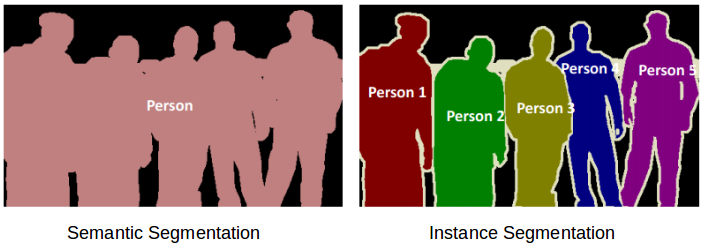
\includegraphics[scale=0.5]{Chapter2/figs/semantic_vs_instance_segmentation.png}
	\end{center}
	\caption{An example showing the difference between semantic and instance segmentation. In semantic segmentation, all pixels which belong to the \texttt{person} class have been classified as one \texttt{person} object. In instance segmentation, five \texttt{person} objects have been detected, and all \texttt{person} pixels have been assigned to one of the objects. Image from \cite{sharma_image_2019}.}
	\label{fig:instance-vs-semantic}
\end{figure}

As such, instance segmentation provides a far more detailed explanation of the input image. This information can be invaluable if the developed system is required not only to understand what pixel classes are present in the input image, but also how many of these class instances there are. In a sense, instance segmentation can be seen as combining both object detection and semantic segmentation into one task. Traditionally however, in order to achieve the goal of instance segmentation, proposed systems have kept the two tasks divided. These \textit{traditionalist} methods take one of two approaches. 

The first, known as \textit{top-down}, begins by detecting objects of interest via an RPN to create bounding boxes. These detections are then fed to the mask predictor to determine which pixels inside of the box belong to either the target or background class. Examples of \textit{top-down} approaches include Faster R-CNN \cite{ren_faster_2015}, and Mask R-CNN \cite{he_mask_2017}. In contrast, \textit{bottom-up} systems first segment then detect, such as SpatialEmbedding \cite{neven_instance_2019} which attempts to tackle instance segmentation through the use of a Gaussian function to produce a probability for a pixel being part of the background or foreground, and then performing object detection on the foreground pixels. \textit{Bottom-up} approaches often fail to reach similar levels of performance as \textit{top-down} approaches however, and are thus rarely used. The major similarity between both \textit{top-down} and \textit{bottom-up} approaches is that they are both sequential in nature, requiring one stage to happen before the other. As such, these systems are very hard to speed up and are far from real-time. However, two stage systems often perform the best in terms of accuracy, and thus are still extremely common backbones of systems requiring the use of instance segmentation. 

In recent years research into the development of real-time instance segmentation has shifted to utilising a one stage approach. These one stage systems are often able to achieve near real-time performance, although often do not produce levels of segmentation accuracy seen when utilising two stage systems. ExtremeNet \cite{zhou_bottom-up_2019} works to extract four "extreme points" and one "center point" of potential objects in the input image through the use of a keypoint estimation network, creating a coarse mask. ESE-Seg \cite{xu_explicit_2019} utilises the concept of Chebyshev polynomials to fit a radius around each object inside of the detected bounding box. Similarly, PolarMask \cite{xie_polarmask_2020} also represents masks through the use of a contour around the object, modelling this through the use of polar coordinates. FourierNet \cite{riaz_fouriernet_2020} builds on this radius concept further through the use of a Fourier transform to smooth the contour. This contouring of the object is extremely fast, however the generated masks are very imprecise. Further, any objects which contain spaces or holes, such as doughnuts, would not be able to be accurately represented. 

YOLOACT \cite{bolya_190402689_2019} builds on the well known YOLO object detection architecture, specifically YOLOv3 \cite{redmon_yolov3_2018}, adding a branch for mask prediction, but performing this through the use of two parallel tasks. The first utilises an FCN to generate prototype masks, whilst the second predicts instance coefficients. These can be combined into one mask through matrix multiplication operations with the detected bounding box. BlendMask \cite{chen_blendmask_2020} works in a similar way to YOLOACT however predicts an attention map rather than instance coefficients and utilises FCOS \cite{tian_fcos_2019} as a backbone, a completely anchor and proposal free object detection architecture resulting in reduced complexity when compared to YOLO \cite{redmon_you_2016} and SSD \cite{liu_ssd:_2016}. 

Whilst the majority of one stage approaches to instance segmentation rely on bounding boxes, this is not always the case. SOLO \cite{wang_solo_2020} introduces the concept of instance categories, assigning categories to each pixel according to the size and location of the instance. SOLOv2 \cite{wang_solov2_2020} builds on SOLO through the implementation of an novel non-maximum suppression algorithm. SOLOv2 often depicts higher quality masks than more often used two-stage systems such as Mask R-CNN and is able to perform real-time inference, although it should be noted that both SOLO and SOLOv2 are extremely recent additions to the instance segmentation arsenal, both being released in 2020. 

\subsubsection{Mask R-CNN}\label{ch:Background,sec:instanceSegmentation,sub:Mask R-CNN}

As discussed in previous Sections, there are multiple standardised architectures utilised for segmentation tasks. As such, when developing a system which utilises segmentation developers of these systems will, more often than not, use one of the many architectures from literature rather than developing their own custom architecture. Utilising one of the standard architectures has many advantages; for one, researchers do not need to spend time creating a model architecture for their task, allowing for development in other, novel areas. Further to this, utilising a standard architecture allows for research to be more easily understood and reproduced. As this thesis focusses on the automation of photo-identification systems rather than on the development of new novel architectures, it makes sense to make use of an architecture which is well known, has a track record of performing well when trained on non-benchmark or custom datasets, and is easily reproducible. As such, parts of this project's automation pipeline make use of Mask R-CNN \cite{he_mask_2017}. Because of this, it is important to understand Mask R-CNN in more detail compared to the other architectures discussed previously in this Chapter. 

As we have seen previously, it is often the case that new architectures either extend or borrow features from older ones. This is also the case with Mask R-CNN. Developed in 2017 by He \textit{et al.} at Facebook AI Research, Mask R-CNN was developed on top of the existing 2016 Faster R-CNN architecture from Ren \textit{et al.} \cite{ren_faster_2015} (itself an extension of Fast R-CNN developed in 2015 \cite{girshick_fast_2015}). 

Faster R-CNN is a two stage architecture. The first stage utilises a standard backbone network, typically ResNet \cite{he_deep_2015}, VGG \cite{simonyan_very_2015}, or Inception \cite{szegedy_going_2015}, to convert an input image into a set of feature maps which are passed to an RPN for analysis (see Section \ref{ch:Background,sec:objectDetection,sub:RPN} for a breakdown of RPNs). This RPN generates region proposals which are passed to the second stage of Faster R-CNN, along with the previously generated feature maps, and fed to an RoI pooling layer.  Here, each proposed region and corresponding feature map is utilised to predict bounding boxes, classifications, and confidence scores. A visual representation of Faster R-CNN's architecture can be seen in Figure \ref{fig:faster-r-cnn-architecture}.


\begin{figure}
	\begin{center}
		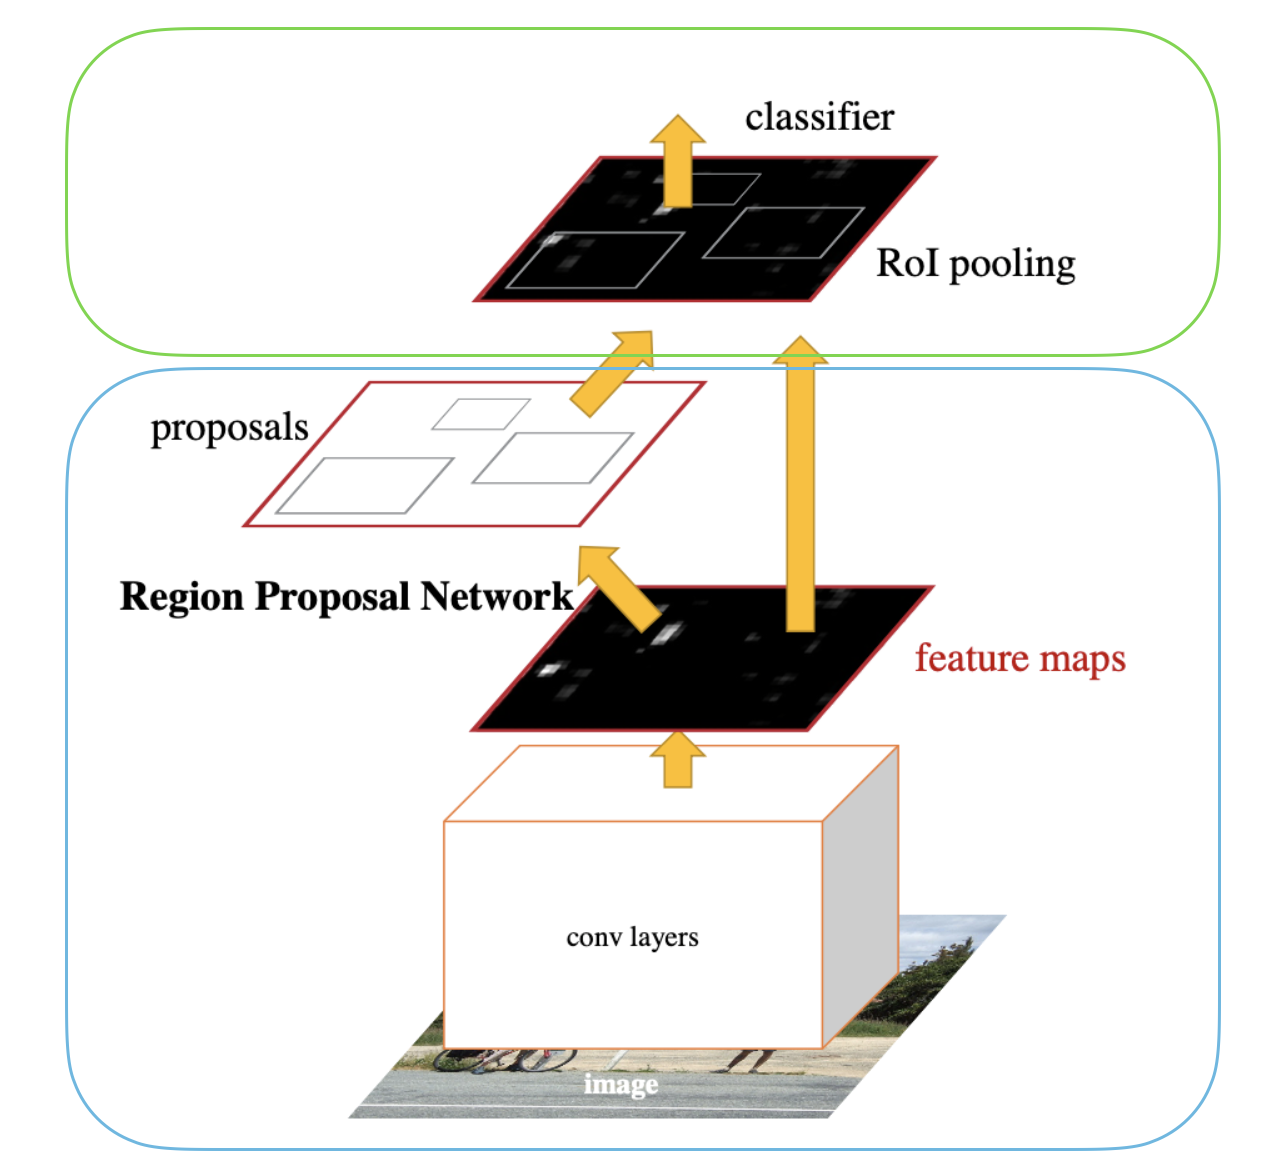
\includegraphics[scale=0.3]{Chapter2/figs/faster-r-cnn-architecture.png}
	\end{center}
	\caption{The Faster R-CNN architecture \cite{ren_faster_2015}. The blue box represents operations in stage one. The green box represents operations in stage two.}
	\label{fig:faster-r-cnn-architecture}
\end{figure}


Mask R-CNN extends Faster R-CNN, allowing for instance segmentation through some relatively simple changes and additions to stage two of the architecture. First, the RoI pooling layer is replaced with an RoI align layer. This replacement layer removes the "harsh quantisation" which is present in RoI pooling, and properly aligns the extracted features with the input image. Second, an additional branch is added to the end of stage two. This branch receives the output of the new RoI align layer and processes it using a \textit{mask head}, consisting of additional convolutional layers which generate pixel predictions and instance mask outputs. See Figure \ref{fig:mask-r-cnn-changes} for a visual representation of the changes made by Mask R-CNN.  

\begin{figure}
	\begin{center}
		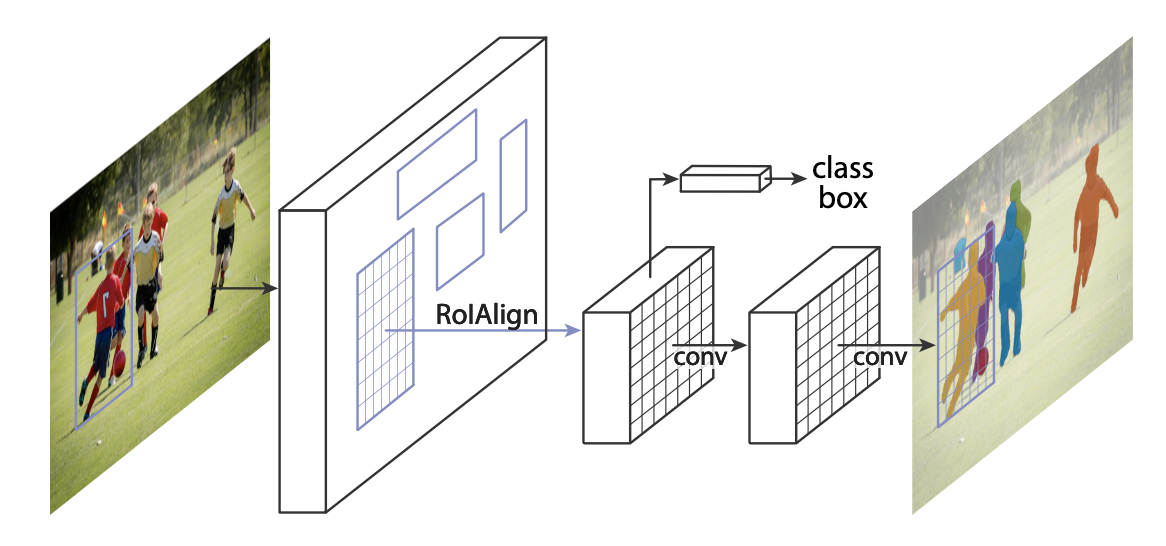
\includegraphics[scale=0.3]{Chapter2/figs/mask-r-cnn-changes.png}
	\end{center}
	\caption{A visual representation of the changes made to Faster R-CNN to create Mask R-CNN. \cite{he_mask_2017}}
	\label{fig:mask-r-cnn-changes}
\end{figure}

Thanks to these additions, Mask R-CNN is able to perform extremely accurate instance segmentation with a relatively small drop in inference speed. Whilst it is not real-time, this is an acceptable trade off for the accuracy of predictions on custom datasets. Indeed the use of Mask R-CNN for instance segmentation in literature is far ranging, being utilised in medical \cite{rohit_malhotra_autonomous_2018, chiao_detection_2019, liu_segmentation_2018, anantharaman_utilizing_2018}, agriculture \cite{qiao_cattle_2019, zhao_comparing_2018, lee_potato_2020, chu_deepapple_2020}, sports \cite{buric_ball_2018, pobar_detection_2019, nguyen_hand_2018}, astronomy \cite{burke_deblending_2019}, and nautical \cite{nie_inshore_2018, hong_trashcan_2020} fields. As well as being well known, Mask R-CNN is also extremely reproducible. An official PyTorch implementation is available through Facebook AI Research's Github \cite{wu_detectron2_2020}, whilst Matterport's Mask R-CNN implementation is most commonly utilised when working with Tensorflow (including in this project) \cite{waleed_mask_2017}.

\subsection{Fine-Grained Visual Categorisation}\label{ch:Background,sec:Fine-grainedCV}

Categorisation of objects through the use of machine learning may at first glance look like a solved problem. Indeed, it is now possible to achieve extremely high levels of accuracy on a wide variety of tasks; at the time of writing the current state of the art for ImageNet \cite{institute_of_electrical_and_electronics_engineers_2009_2009} and CIFAR-10 \cite{krizhevsky_learning_2009}, two of the most commonly used classification benchmark datasets, are both held by Foret \textit{et al.} utilising EfficinetNet with SAM \cite{foret_sharpness-aware_2020} at 88.61\% and 99.70\% top-1 accuracy respectively. Even outside of these benchmarks however, high accuracies would be expected for more complex use cases where custom datasets have been created, such as in manufacturing environments. However, it is important to note that all of these tasks are coarse-grain in nature. Benchmark datasets usually contain classes which are relatively distinct, for example \texttt{cat}, \texttt{dog}, and \texttt{ship} classes in CIFAR-10, which all have large interclass variation. 

In more recent years the focus of research in object detection has thus mostly shifted from the coarse-grain to the fine-grain domain, where distinct classes have small interclass variation. For example whilst CIFAR-10 has one class covering all different types of \texttt{dog}, the fine-grain dataset Stanford Dogs \cite{khosla_novel_2011} is made up of 120 classes each containing examples of only one dog breed each (\texttt{chihuahua}, \texttt{beagle}, etc.). Other common fine-grain benchmark datasets often focus on wildlife or vehicles, including Caltech-UCSD Birds 200 \cite{welinder_caltech-ucsd_2010} and the updated Caltech-UCSD Birds 200-2011 \cite{wah_caltech-ucsd_2011}, iWildcam for camera trap data \cite{beery_iwildcam_2019}, and FGVC Aircraft \cite{maji_fine-grained_2013}. 

Whilst fine-grain datasets may contain small inter-class variation, their intra-class variation is often large. Class examples often contain a wide variety of orientations, poses, colour, and sizes. This allows for trained models to be more generalisable and capable of detecting class examples in previously unseen images where the example may be obscured or unlike conventional class examples. It is also important to note here that models which perform well on coarse-grain data are not guaranteed to do so on fine-grain data. For example EfficientNet with SAM which, as previously stated, is state of the art in multiple coarse-grain tasks currently ranks 31\textsuperscript{st} in the FGVC Aircraft benchmark ranking on Papers With Code \footnote{Papers With Code - FGVC Aircraft Rankings: \href{https://paperswithcode.com/sota/fine-grained-image-classification-on-fgvc}{paperswithcode.com/sota/fine-grained-image-classification-on-fgvc}}.

\section{Computer Vision for Conservation Technology}\label{ch:Background,sec:conTech}

Thanks to the large advancements in computer vision and deep learning, and the increasing prevalence of these systems in areas such as manufacturing and healthcare, researchers have, in recent years, began exploring other areas of society which could benefit from AI systems. One of the more niche, but arguably highly important areas where computer vision can make an impact, is conservation \cite{weinstein_computer_2018}.

Work in conservation tech has been mostly dominated by machine learning systems for camera traps. This makes sense, as this data collection technique usually operates over vast spatial and temporal areas. As such, a large amount of varied data already exists for systems to be trained on. For example, the Snapshot Serengeti project \footnote{Snapshot Serengeti: \href{https://www.snapshotserengeti.org/}{snapshotserengeti.org}}, developed by Swanson \textit{et al.} has utilised camera traps in Tanzania's Serengeti National Park to develop a fully labelled camera trap image dataset capable of training machine learning systems. The camera traps used have been in continuous operation since 2010 and cover an area of 1125km\textsuperscript{2} \cite{swanson_snapshot_2015}. The iWildcam dataset provides further camera trap training data from across the South-western United States \cite{beery_iwildcam_2019}.

 A second advantage of camera trap data is their high false positive rate. These traps capture a photo every time movement in the frame is detected, and as such a large proportion of the images a camera trap captures either do not contain any animals at all (e.g. wind has caused the surrounding vegetation to move), or contain animals which are not the primary species of investigation. This large false positive rate provides a key driver for the development of machine learning camera trap systems which could, for example, filter out these false positive captures automatically. Whilst these images may simply be discarded by the researchers, they have a use in the development of machine learning camera trap based systems, allowing the system to be trained on a wide variety of false positive examples. As such, machine learning systems developed for camera traps have found quick adoption in the conservation community with many systems now capable of performing fine-grained species classification with extremely high accuracy \cite{tabak_machine_2019, norouzzadeh_automatically_2018, willi_identifying_2019, beery_efficient_2019, norouzzadeh_deep_2019}. Recent work by Clapham \textit{et al.} has moved further to the extreme of fine-grained classification with BearID, a project which adapts human facial recognition systems for use with brown bears (\textit{Ursus arctos}) via metric embeddings, achieving an ``individual classification accuracy'' of 83.9\%. Here, BearID is not classifying the species \textit{Ursus arctos} but rather individuals within the \textit{Ursus arctos} population, a significant achievement given the challenge of identifying individuals within a species which do not have unique markings \cite{clapham_automated_2020}.

Marine conservation researchers, in contrast to their on-land counterparts, have been slower at adopting computer vision to aid their research. This is, in part, due to the relative lack of available data to train systems. Due to the unsuitability of marine environments for the deployment of camera traps, conservationists here traditionally rely on identification from photographs taken either from the coastline or from a vessel. As this requires a human operator, the size of datasets available is relatively small. Furthermore, given the high cost of data collection, marine conservation groups often keep a tight grip on their data. This has led to a lack of available open-source datasets for those who wish to train machine learning systems for use in marine conservation. Thanks to advances in UAV technology and their current inexpensiveness, some research groups have shifted focus to the use of drones for image capture. This new approach has seen success in areas such as photo-identification \cite{bogucki_applying_2019, gray_drones_2019}, microbial sampling \cite{centelleghe_use_2020}, and human-interaction response monitoring \cite{fiori_using_2020}. The use of drones for this time of work is not yet mainstream however, and some recently published work highlights the need to better understand how drones affect the behaviour and health of marine species \cite{giles_responses_2020, bevan_measuring_2018, ramos_bottlenose_2018, pomeroy_assessing_2015}. 

\subsection{Utilising Computer Vision in Cetacean Conservation}\label{ch:Background,sec:conTech,sub:cetaceanDetection}

The idea of utilising statistical methodology and machine learning in a marine cetacean space has, in recent years, been gaining popularity, with multiple papers being published in this area. Karnowski \textit{et al.} propose using Robust PCA to subtract background from underwater images to help identify captive bottlenose dolphins, and track their movements through multiple distinct areas, allowing researchers to annotate pool positions 14 times faster than before \cite{karnowski_dolphin_2015}. Bouma \textit{et al.} provide a system focusing on metric embedding learning to photo-id individual common dolphins, achieving top-5 accuracy scores of around 93\% \cite{bouma_individual_2018}. Further, Qui\~{n}onez \textit{et al.} propose a CNN based system to detect four classes: \texttt{dolphin}, \texttt{dolphin\_pod}, \texttt{open\_sea}, and \texttt{seabirds} \cite{quinonez_using_2019}. 

Outside of statistical theory and academic papers, multiple systems have been developed, or are currently in development, to aid cetacean researchers in the photo-id process. The first of these, known as FinScan, was developed in 2000 \cite{hillman_finscan_2002}. This is a semi-automated photo-id assistant whereby the user imports images taken during fieldwork which FinScan then attempts to create a trace of the fin in the image. Users may manually edit this trace however if it is not exact (this feature was developed due to frustration with barnacles attaching to fins in the area where FinScan was developed). This trace of the fin is then checked against a local Microsoft Access database to determine close matches which are presented to the user. Before images are imported into FinScan they must be manually cropped, sharpened, and rotated by the user. Rotation of the image is especially important, and the FinScan algorithm is not rotation invariant. Further to this due to FinScan being an old piece of software, whilst it is freeware it is no longer readily available. Anyone who wishes to use it must procure a copy from someone else, there is no central repository for downloading. Issues with running the software on newer systems may also be present.

Similarly to FinScan, FinBase is a photo-id database management system developed by NOAA Fisheries \cite{fisheries_finbase_2018}. However, unlike other systems, FinBase provides no matching based on automatically generated fin properties; instead, FinBase facilitates matching through user defined attributes. These could be physical descriptors such as `top notch' or `skin disorder' but may also be non-physical attributes if the user wishes. Fins are partially matched based on querying the backend database for entries which also have the attributes of those inputted by the user for the query fin. 

Alongside both of these, DARWIN \cite{hale_unsupervised_2012} provides automated identification of new images based on those already in the attached database. Like FinScan, users of DARWIN trace around the leading and trailing edges of the fin they wish to identify. These edges are stored in a database as a set of evenly spaced points approximating the outline of the fin which is then used for identification.

Photo-ID Ninja\footnote{Photo-ID Ninja: \href{http://photoid.ninja}{photoid.ninja}} is a system currently in development which aims to photo-id individuals based on pigmentation commonly found on fins of the New Zealand common dolphin (\textit{Delphinus} spp.) \cite{gilman_computer-assisted_2016}. Here, pigmentation is used due to the low chance of other prominent markings becoming present on individuals. Matching is performed via the Euclidean distance between the input image and the catalogue of known individuals, which is then sorted by ID and validated using 5 fold cross-validation \cite{bouma_individual_2018-1}. Current reported accuracies for this pigmentation matching are a top-1 accuracy of 90.6\%, top-5 accuracy of 93.6\%, and an mAP of 80.8\%. This pigmentation matching is still in development however, although Photo-ID Ninja does currently provide a bulk cropping mechanism to aid in the speed up of manual identification. Users can provide a batch of images taken directly from the field to the system, which then outputs a zip file of cropped fins which can then be manually identified. 

Work undertaken by Georgetown University and Google in the area of cetacean photo-id has also provided promising results \cite{mann_mann-urian-google_2019, georgetown_university_is_2018, liang_googles_2018}. The system, which utilises Google's Cloud Auto ML framework, can quickly identify bottlenose dolphins from Australia's Shark Bay. This system shows users the top-200 closest matches along with their confidence scores utilising both the leading and trailing edges of the fin. It is reported that this system saves Georgetown University's cetacean team around 4500 hours per year, highlighting the need for systems such as these to researchers in this field. However, this system does not link to a backend database to log matches found - this must be done manually by the researchers. Further, any new individuals which need to be added to the system, or indeed if the system was to be redeployed to a new area, then all training of the underlying model must be performed by Google engineers rather than locally by the researchers who wish to utilise the system. Further, fins to be identified must be inputted one by one, no batch input function exists.  

In the past few years, systems utilising CNNs have started to enter the photo-id space. HappyWhale\footnote{HappyWhale: \href{https://happywhale.com/}{happywhale.com}} is a CNN based photo-id system focussing on humpback whales (\textit{Megaptera novaeangliae}). The underlying CNN for this system was developed through a Kaggle competition\footnote{Kaggle competition: \href{https://www.kaggle.com/c/whale-categorization-playground}{kaggle.com}} by user Jinmo Park to identify patterns present on the tailstock of the humpbacks \cite{kaggle_humpback_2018}, utilising elements of ArcFace \cite{deng_arcface_2019} and DeepFace \cite{taigman_deepface_2014} to do so. Users interact with HappyWhale through their website, uploading images of the tailstocks encountered. The HappyWhale system then attempts to identify the individual before presenting back to the user. If the user provides location data, HappyWhale also keeps track of this to produce travel maps for the individuals, as humpback whales are known to travel vast distances in their lives. Success rate for HappyWhale varies greatly, from 99\% for "good to high quality" images to 50\% for full fins at 50x50px. HappyWhale struggles with partially obscured tailstocks however, and work is currently ongoing in this area \cite{cheeseman_happywhale_2019}. 

Of all the systems in use or development today, one of the largest and most well known is FlukeBook\footnote{FlukeBook: \href{https://www.flukebook.org/}{flukebook.org}}, a fully automatic photo-id system for bottlenose dolphins, humpback whales, and sperm whales (\textit{Physeter macrocephalus}). This system is part of a wider network of animal identification tools based on Wildbook, an open source software framework developed by non-profit organisation WildMe to facilitate the introduction of artificial intelligence into the conservation space \cite{berger-wolf_wildbook:_2017}. Within FlukeBook there are two main photo-id algorithms; CurvRank and FinFindR.

CurvRank is an algorithm developed by Weideman \textit{et al.} \cite{weideman_integral_2017} which automatically identifies the trailing edge of the fin and represents this as a set of ordered coordinates. Each coordinate point then has a circle of radius $r$ placed upon it, before being transformed horizontally. The curvature at this point for a given $r$ value is then defined as the ratio of the area under the curve againsy the area of a square around the curve of length $2r$. This allows for the definition of the trailing edge of the fin to be rotation invariant. 

FinFindR is an algorithm developed by Thompson \textit{et al.} which allows for inputted images containing bottlenose dolphins to be identified. FinFindR works with uncropped images of the whole area unlike other systems which require just the fin to be in the image. FinFindR then automatically detects the dolphin and crops it out, saving a new image. Cropping can be performed on either the whole body or on the dorsal fin only. This cropped image is then passed to a canny edge detector which creates an embedding of the trailing edge of the fin. This embedding is mapped into a high dimensional space based on work in FaceNet \cite{schroff_facenet_2015}, with clustering of individuals achieved using Ward's variance minimising clustering \cite{ward_hierarchical_1963}. Reported accuracies for FinFindR currently stand at a top-1 accuracy of 88\%, top-5 accuracy of 94\%, and top-50 accuracy of 97\% \cite{thompson_finfindrpdf_2019}. It should be noted however that FinFindR has currently only been tested on bottlenose dolphins and work is still ongoing. The code for FinFindR can be found on GitHub \footnote{FinFindR: \href{https://github.com/haimeh/finFindR}{github.com/haimeh/finFindR}}.

Recent work undertaken by Lee \textit{et al.} proposes a novel algorithm for cetacean identification \cite{lee_backbone_2020}. The proposed system is capable of detecting small objects in large images, and utilises this for fin detection. Next, segmentation is performed using U-Net \cite{ronneberger_u-net_2015}. The resultant output is then passed to a post processor which re-aligning and normalising the fin. The most significant features of the fin are then extracted and passed to a VGG based system \cite{simonyan_very_2015}, combined with a novel V2BC component, for identification. 

Maglietta \textit{et al.} propose DolFin \cite{maglietta_dolfin_2018}, a SURF based system \cite{bay_speeded-up_2008} building upon work undertaken by Renò \textit{et al.} \cite{reno_sift-based_2019} for identifying Risso's dolphins. As mentioned in Section \ref{ch:Background,sec:photo-id}, this species is susceptible to prominent long-term scarring, and thus is well suited to feature detection algorithms such as SURF, with published results showing a much greater identification accuracy can be achieved compared to utilising common photo-id aides such as DARWIN \cite{hale_unsupervised_2012}.  

Morteo \textit{et al.} \cite{morteo_phenotypic_2017} perform semi-automatic fin measuring using FinShape in order to aid in population monitoring. This technique, based on \cite{weller_global_1998}, does not require the user to trace the fin; instead lines are projected out from the base of the leading edge of the fin, with the user cutting these lines where they intersect with a point on the trailing edge. 

\section{Summary}\label{ch:Background,sec:Summary}

This Chapter presents the key ideas required to understand and appreciate the novel work proposed in this thesis. An extensive overview of deep learning and computer vision is provided, as well as an introduction to photo-id, a key methodology for mark-recapture surveys utilised by conservationists. A summary of previous research combining conservation and deep learning has also been provided, with a focus on marine environments and cetaceans. 

The ability to perform object detection on photo-id fieldwork data to identify regions in images where cetaceans are present is a key component of this thesis. Chapter \ref{ch:cetDet} will discuss this work in more detail, including an in-depth analysis of the cetacean detector's requirements, as well as its implementation and evaluation.

%%%%%%%%%%%%%%%%%%%
\nomenclature[z-CNN]{CNN}{Convolutional Neural Networks}
\nomenclature[z-CV]{CV}{Computer Vision}
\nomenclature[z-CPU]{CPU}{Central Processing Unit}
\nomenclature[z-GPU]{GPU}{Graphical Processing Unit}
\nomenclature[z-SGD]{SGD}{Stochastic Gradient Descent}
\nomenclature[z-ReLU]{ReLU}{Rectified Linear Unit}
\nomenclature[z-FCN]{FCN}{Fully Convolutional Network}
\nomenclature[z-RPN]{RPN}{Region Proposal Network}

\chapter{Cetacean Detection Using Deep Learning}\label{ch:cetDet}

When building any large-scale project, it is important to break the task down into various subcomponents. This Chapter examines one such subcomponent utilised in the development of an automatic photo-id system, the cetacean detector. This component takes images captured during photo-id surveys and detects regions of interest - dorsal fins which have breached the waterline. This Chapter will discuss the requirements a detector must meet, as well as its training and hyperparameter optimisation. 

\section{Requirements of a Cetacean Detector}\label{ch:cetDet,sec:requirements}

Before a system for automatic cetacean detection can be developed, it is important to first define the problem and understand the requirements of the system. The overall aim of the detector is to be able to take large-scale images as input, fed in one at a time, and process them in order to locate regions of interest (RoIs). This detector will only be required to identify one object class, \texttt{dolphin}. These detected regions can then be passed further down the system pipeline for photo-identification. 

 As such this detector can be considered a coarse-grain task, and at first glance may seem somewhat trivial. However due to both the nature of the environment in which the RoIs must be detected in, and the technical requirements the system must perform under, this is actually a complex problem. 
 
 \subsection{Environmental Requirements}\label{ch:cetDet,sec:requirements,sub:environmental}
 
 First the area in which this system is to be deployed, open water, is susceptible to adverse weather conditions such as high winds. This in turn leads to sub-optimal conditions for detection which the system must be capable of handling, most notably high amounts of sea swell. Further to this, cetaceans are communal and travel in pods. An example of this behaviour can be seen in Figure \ref{fig:pod-eg}. Thus, the system must be capable of differentiating between overlapping individuals. Even if not all of the overlapping individuals are suitable for identification downstream, the system must still be able to separate them into individual detections to prevent further misclassification downstream.
 
 \begin{figure}
 	\begin{center}
 		\includegraphics[scale=0.06]{Chapter3/figs/dolphins-in-pod-example.JPG}
 	\end{center}
 	\caption{Some cetaceans, such as bottlenose dolphins, travel in pods. The developed detection system must be capable of splitting this pod into individual animals to be passed to the identifier.
 	}
 	\label{fig:pod-eg}
 \end{figure}

 Next, the detector must be capable of differentiating between dolphin fins and waves. Again this might sound trivial, but thousands of years of evolution have resulted in fins and waves looking extremely similar to the untrained (artificial) eye. Especially from a distance and in choppy waters, fins and waves often have extremely similar shape and dimensions. Furthermore, the animal's bodies are also similarly coloured to their surroundings. These adaptations allow the animals to be better protected and camouflaged in their environment, but can cause issues with detection systems. This becomes apparent when thinking about how CNNs \textit{see}. As described in Chapter \ref{ch:Background,sec:DLforCV}, CNNs see input images as a matrix of pixel values. When training an object detection system the CNN is also told which parts of this matrix are related to a class, any without a class label are considered background. If fins and areas of background contain similar pixel values, and these pixel values are clustered in similar ways, this can result in issues when training a model to detect instances of a class without misclassifying the background. 
 
 Another important requirement is for the detector to be able to handle objects of varying size, shape, direction, and angle of approach. When working in an open water environment with live animals, there is no guarantee how the animal will approach the camera, and thus the detector must be generalisable enough to handle this. 
 
 Furthermore how the animals breach the water is also extremely variable. Breachings may occur in any direction relative to the boat and the animal could itself be travelling in a different cardinality. The ideal scenario in this case would be for a breaching to occur either directly East or West of the boat (off the port or starboard side respectively) with the animal travelling perpendicular as this provides the best chance of marking capture, however this rarely occurs. For example, a breaching may occur off the port-side of the bow (approx North West relative to the boat), but the animal may be travelling in a South-Easterly direction. These approaches greatly change the look of the fin, however they may still contain identifiable markings. The detector should be able to detect these fins and pass them along for identification. An example of this can be seen in Figure \ref{fig:angle-eg}, which also shows how distance from the vessel can change the camera's view of the dorsal. 
 
   \begin{figure}
 	\begin{center}
 		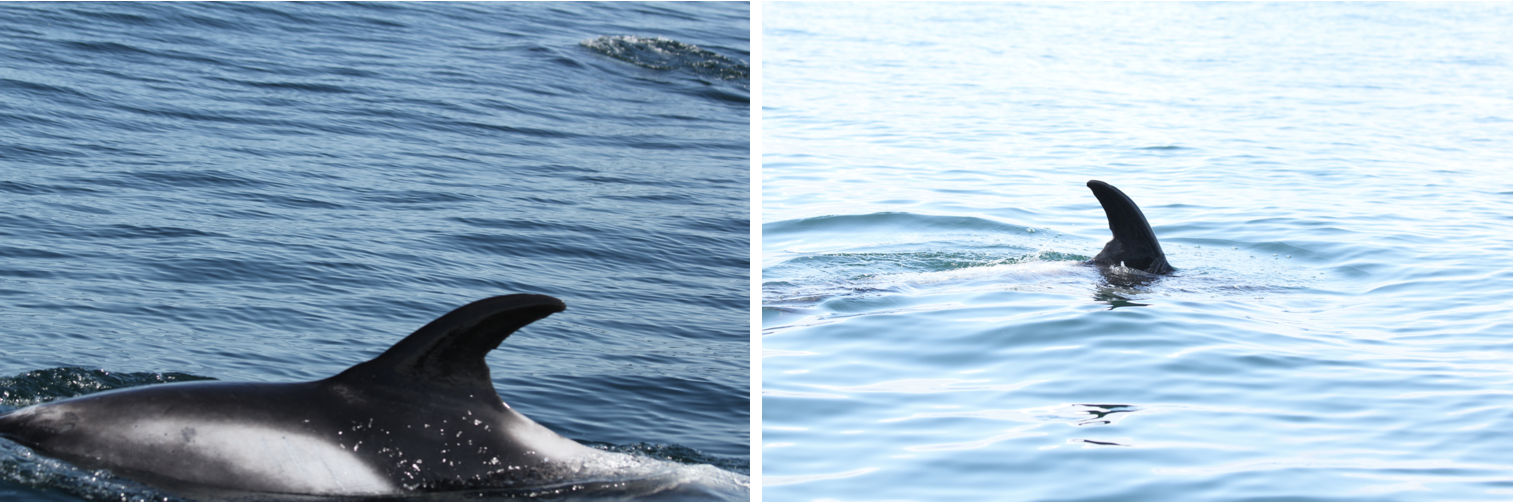
\includegraphics[scale=0.6]{Chapter3/figs/angle-size-example.png}
 	\end{center}
 	\caption{Two images of the same individual taken from different angles of approach, directions of travel, and distances from the vessel. Note how this changes the make-up of the dorsal fin but keeps the identifying notch visible. 
 	}
 	\label{fig:angle-eg}
 \end{figure}
 
 As mentioned previously, weather conditions can also greatly affect how a dorsal fin is captured by a camera. However in photo-id surveys there are only two conditions that need to be worried about; swell and lighting. This is due to most research groups limiting travel in rough seas for safety reasons. With regards to Newcastle University's Marine MEGAfauna Lab, this limit is a sea state less than 3 on the Beaufort scale \cite{world_meteorologicial_society_beaufort_1970}. As such, a mild amount of swell and splash can be expected which the detector should be capable of handling. Lighting conditions are not considered in the Beaufort scale, but for operational reasons the vast majority of photo-id surveys take place during daylight hours. This can lead to large amounts of glare in images, especially on clear days. The detector should be invariant to these conditions. 
 
 \subsection{Technical Requirements}\label{ch:cetDet,sec:requirements,sub:technical}
 
On top of being able to handle a variety of environmental factors, there are also some technical requirements that the detector must meet. With all deep learning based computer vision approaches, there is often a trade off that must be made between speed and accuracy. In most cases, these are inversely proportional to each other; the faster a system is required to perform, the lower an accuracy you must be willing to tolerate - Huang \textit{et al.} discuss this in greater detail \cite{huang_speedaccuracy_2017}. Thanks to the pace of research in this area, 2020 saw the release of detection architectures which can perform operations in real-time such as EfficientDet \cite{tan_efficientdet_2020} and YOLOv4 \cite{bochkovskiy_yolov4_2020}. Current accuracies on benchmark datasets using these real-time architectures are still a long way off their non-real-time competitors however, and accuracies would drop further on custom non-benchmark tasks such as cetacean detection. 
 
 Because this trade off must be made, before deploying a deep learning model it is important to decide where the system will be utilised. As photo-id surveys are performed on small vessels such as RIBs, space is severely limited on board. Because of this, it is not appropriate to add additional hardware to the vessel to perform this analysis during the survey. Furthermore, the current methodology of cetacean researchers is to perform identification once back on land, even when utilising photo-id aides. As the system proposed in this project is intended to fit into existing procedures rather than replace researchers, it is appropriate for the system to also be land based rather than on the vessel. Thinking about the current procedure further, this project's proposed system could be, for example, left running overnight performing identifications whilst the researchers are asleep or during the day whilst they are on surveys. As such, there is no need for the system to operate in real time to fit in with the current workflow of cetacean researchers provided the system completes its task within a reasonable time frame. Further to this, as the output of the detection model will be passed to an identification module, it is imperative that as much noise is removed as possible during the detection. In order to do this, the accuracy of the detection must be as high as possible, furthering the case for an accurate system over a fast one.
 
 This idea of reducing as much noise as possible can be used to further narrow down the requirements of the detection system. As discussed in Section \ref{ch:Background,sec:DLforCV}, the output of detection systems can be provided in different formats. In bounding box detection systems the detected objects are described by a set of at least two pixel coordinates denoting the top-left and bottom-right extremes of the object. These detections are often more cost-effective, both from a labelling perspective requiring less person-hours to complete, and to perform computationally. Bounding box based detections are limited in their ability to remove background noise however, with only the background outside of the box removed.
 
 If we utilise pixel wise mappings however, then each pixel is given a classification. This allows the system to be more discrete with its detection, allowing for the removal of as much background as possible. Both semantic and instance segmentation methods allow the detector to utilise pixel-wise mappings to remove background noise. Pixel wise labelling is far more labour intensive and costly to produce compared to bounding box labelling, and systems capable of pixel level detections are often slower than bounding box detectors. Utilising our requirements as defined in Section \ref{ch:cetDet,sec:requirements,sub:environmental}, specifically that the detector must be capable of reducing an overlapping pod to its individual component animals, the use of pixel wise mappings at an instance level would be preferable over semantic or bounding box level detections. This requirement reveals a further trade-off the system must make. The amount of noise removed by the detector is proportional to the cost and labour needed to create data to train the system. This is discussed in more detail in Section \ref{ch:cetDet,sec:deciding,sub:boundingBoxInvestigation}.
 
 Furthermore, any system performing cetacean detection from photo-id survey data must be capable of working with large scale images. In most image based tasks where deep learning is utilised images fed to the network are downscaled, typically to sizes such as 224x224 to allow for faster training and a reduction in overall network size. Downscaling images reduces the number of pixels in the image, which by definition reduces the amount of information present as pixels values need to be pooled (one pixel needs to now display what multiple would have previously). For most detection tasks this would not be an issue, and indeed if this project was solely a cetacean detection task there would be no issues with downscaling. This detector is not stand-alone however but rather the first stage of a pipeline of networks with the end goal of photo-identification. The identification task relies on potentially minute details in the fin such as notches; any downscaling of the image at the detection stage runs the risk of removing potentially identifiable information in the fin. As such, the image must only be reduced in size once it is certain that no identifying information will be lost. As this cannot be guaranteed at the stage of detection, the detector must be capable of operating on images without resizing.
 
\section{Deciding on Architecture and Framework}\label{ch:cetDet,sec:deciding}

Based on the requirements outlined in Section \ref{ch:cetDet,sec:requirements}, it is possible to begin deciding on how the cetacean detector is to be developed. One of the most important factors in the overall approach taken in the detector's development, and ultimately the overall automatic photo-id system, would be the use of either bounding boxes or pixel-wise mappings. As mentioned previously, the use of pixel-wise mappings would allow for a greater removal of background noise, but is extremely costly and labour intensive to produce. In contrast, bounding box labels are easier and cheaper to produce but will lead to less background noise removal. 

\subsection{An Investigation into Bounding Boxes}\label{ch:cetDet,sec:deciding,sub:boundingBoxInvestigation}

Due to their relative cheapness and ease to produce, the use of bounding boxes in this project would be extremely beneficial. However, if the use of bounding boxes at this stage would hinder the accuracy of individual identification downstream, then this would outweigh the cost of pixel-wise mappings. 

As such, an investigation was undertaken to decide whether bounding boxes would be a viable option and if their use would hinder downstream identification. To begin, a small amount of data was provided by the Marine MEGAfauna Lab, discussed in more detail in Section \ref{ch:cetDet,sec:initialTesting,sub:zanzibar}, which contained images captured during a previous cetacean survey. A subset of this data was manually cropped to simulate the output of a bounding box detector, an example of which can be seen in Figure \ref{fig:manual-crop-example}. This manually cropped data included some background but ensured the RoI, the dorsal fin, was centred and prominent representing an optimal output from a bounding box detector. 

\begin{figure}
	\begin{center}
		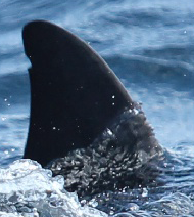
\includegraphics[scale=0.6]{Chapter3/figs/manual-crop-example.png}
	\end{center}
	\caption{An example manual crop utilised in bounding box suitability testing.
	}
	\label{fig:manual-crop-example}
\end{figure}

\subsubsection{Feature Extraction with SIFT}\label{ch:cetDet,sec:deciding,sub:boundingBoxInvestigation,subsub:SIFT}

To begin, processing of the cropped images focussed on the use of feature extractors such as Scale-Invariant Feature Transform, also known as SIFT \cite{lowe_object_1999}. As the name suggests SIFT is invariant to scale, a major advantage for use with cetacean survey data where the RoI's size may change depending on when the image of the dorsal fin breaching the water is captured. If SIFT was capable of producing feature descriptors of the dorsal fins with only partial background removal, this would show potential for individual identification where some background is present, possibly through the use of the feature descriptors.

First SIFT was performed on the entire cropped image, however this proved unfruitful, picking out very few features in areas of the image which contained the animal's dorsal fin and instead focussing on the feature heavy areas present in the sea, even in images containing relatively calm water. This result indicated that further refinement was required, potentially reducing the area SIFT was allowed to explore. 

Reduction of the search space available to SIFT was achieved through the use of colour thresholding. Here, a mask was created programmatically for each image based on bounded RGB colour values found in the dorsal fins, giving an upper threshold of (14, 16, 26) and a lower threshold of (54, 51, 66). As such, SIFT would only be performed in areas of the image where pixel values fell within this range. An example result of SIFT after colour thresholding can be see in Figure \ref{fig:manual-crop-sift-colour-thresholding-example}, with coloured circles surrounding an extracted feature. As can be seen, colour thresholding helps in removing a large amount of background water from the computation. Issues arise however where areas of water are also within this thresholding. Because of this, colour thresholding before SIFT only reduces the amount of features extracted from the water, it does not remove them, which may result in misidentification downstream.

Further to this, it can be seen that SIFT is incapable of extracting relevant prominent markings from the species in the image, Indo-Pacific bottlenose dolphins (\textit{Tursiops aduncus}). For example, in Figure \ref{fig:manual-crop-example}, a notch is clearly present on the dorsal fin which is a good marker for individual identification. However, when performing SIFT on this dorsal as seen in Figure \ref{fig:manual-crop-sift-colour-thresholding-example}, note how this notch has not been detected by SIFT, which has instead detected an area above the notch which contains no identifiable information. 

\begin{figure}
	\begin{center}
		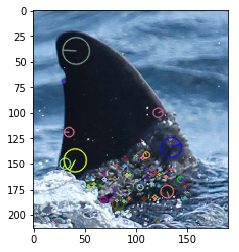
\includegraphics[scale=0.6]{Chapter3/figs/manual-crop-sift-colour-thresholding.png}
	\end{center}
	\caption{An example manual crop showing the result of SIFT feature extraction when thresholded based on RGB colour values.
	}
	\label{fig:manual-crop-sift-colour-thresholding-example}
\end{figure}

Feature extraction methods such as SIFT are also incapable of extracting other identifiable markers such as fin shape. As such, the use of SIFT was deemed improper for this use case. It is important to note here that the use of SIFT may be appropriate for cetacean species other than this project's data subjects of bottlenose and white-beaked dolphins. For example, the use of SIFT has been shown to be appropriate to aid in identification of individual Risso's dolphins by Maglietta \textit{et al} \cite{reno_sift-based_2019}.

\subsubsection{Background Removal with GrabCut}\label{ch:cetDet,sec:deciding,sub:boundingBoxInvestigation,subsub:GrabCut}

Testing the suitability of SIFT as described in Section \ref{ch:cetDet,sec:deciding,sub:boundingBoxInvestigation,subsub:SIFT} highlighted the need for complete background removal before identification would be possible with bottlenose and white-beaked dolphins. In order for bounding boxes to be a viable option in this scenario, a robust background removal process would need to be created. Further, the process would need to be capable of operating under unseen conditions in an unsupervised manner without pixel labelled data to train on. If the background removal process required training data to operate, this would increase the overall cost and labour required to use bounding boxes, and as such reduces the suitability of them compared to utilising pixel-wise mappings from the beginning.

The current state of the art in this area is GrabCut, proposed by Microsoft Research \cite{rother_grabcut_2004}. This algorithm allows for the segmentation of foreground objects from the background with minimal or no human interaction. As GrabCut would be utilised in a fully automated setting, GrabCut would be required to perform background removal with no human interaction. Testing of the suitability for GrabCut was performed using the same cropped images as those used for SIFT testing. Again, issues arose when performing GrabCut on the cropped image data. The algorithm struggled to understand which parts of the image were background and foreground, resulting in imperfect segmentations. This was especially an issue where the dorsal fin was present in rough water, where splash would be in-front of the dorsal fin when captured by the camera. The use of GrabCut on Figure \ref{fig:manual-crop-example} can be seen in Figure \ref{fig:grabcut-example}.

\begin{figure}
	\begin{center}
		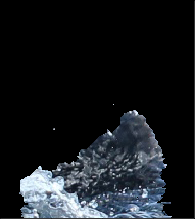
\includegraphics[scale=0.6]{Chapter3/figs/grabcut-example.png}
	\end{center}
	\caption{An example manual crop showing the result of GrabCut background removal.
	}
	\label{fig:grabcut-example}
\end{figure}

As can be seen, the use of GrabCut as a background removal tool does not perform as expected on data the detector is required to operate on. Because of this, as well as the unsuitability of feature extraction as seen in Section \ref{ch:cetDet,sec:deciding,sub:boundingBoxInvestigation,subsub:SIFT}, the use of bounding boxes in the cetacean detector stage was deemed not to be possible. As such, the focus of testing moved to the use of pixel-wise mappings and instance segmentation.  

\subsection{Instance Segmentation Architectures}\label{ch:cetDet,sec:deciding,sub:instanceSegArchitectures}

One of the major decisions that must now be made is which model architecture should be utilised in order to provide the required pixel-level detections. As this project is devoted to improving existing procedures and introducing deep learning to a novel space, it is far more advantageous to utilise existing model architectures rather than develop a custom one. The development of a custom architecture for this stage of the project would be extremely consuming, taking away time from more novel parts of the project (notably the identification of the individual animals). Further, as this project is introducing deep learning methods to a space where it is not commonplace, the project needs to be able to convince researchers in the space that the system is reliable; this is more easily achieved using a pre-existing architecture where use cases already exist in literature and business. 

To this end there are two main model architectures that can be chosen for this task; U-Net \cite{ronneberger_u-net_2015} and Mask-RCNN \cite{he_mask_2017}. Both of these architectures work in different ways. Vuola \textit{et al.} provide a more detailed comparison between the two models \cite{vuola_mask-rcnn_2019}, however the main focus for this project is their resultant output mask structure. 

U-Net is based on an encoder-decoder architecture. This allows for fast and simple segmentation when working with images where you only require one output. For example, taking U-Net's original use case of biomedical imaging, let's assume we have an image showing a group of cells and we wish to segment them into the individual components. U-Net is able to perform this operation efficiently through boundary estimation to locate the outer edges of the cells which allows them to be segmented from each other. However this results in an output of the same dimensions as the input, that is, all segmentations are provided in a single binary mask. 

In contrast, Mask-RCNN utilises a multi-stage architecture (described in more detail in Section \ref{ch:Background,sec:instanceSegmentation,sub:Mask R-CNN}). This allows the architecture to place each detection on its own binary output mask. This is extremely important for our use case; as our detector will be used as part of a larger system, passing information downstream to the identifier which will require individuals to be in their own images, processing each individual in series. If U-Net was utilised for the detection stage, whilst initially being more efficient than Mask-RCNN, further processing of the binary output mask would be required to split this into it's individual components. In contrast, if Mask-RCNN was utilised then the processing required in between the detection and identification stage would be far simpler. Again, this allows for more time to be spent working on the novel aspects of this project whilst keeping the pipeline as simple as possible. This reason was a big factor in deciding to focus on Mask-RCNN for this stage.

Another factor which must be decided upon when starting development of a deep learning system is the language and framework to be used for development. With regards to language this was a fairly easy decision; the vast majority of deep learning research and development is written in Python. The language benefits from an efficient and lightweight syntax as well as having a host of different deep learning packages available to aid in development. Further to this, both of the major deep learning frameworks, Google's Tensorflow \cite{abadi_tensorflow:_2016} and Facebook's Torch (of which PyTorch is the most actively developed) \cite{paszke_automatic_2017}, both provide full Python support and have active communities for the language. Thanks to this, the vast majority of deep learning development is performed using Python in one of these two frameworks. By utilising these technologies, this project's code is easily reproducible and understood, as well as extendable in the future.

Of the two main frameworks, the use of Tensorflow was decided for the project at this stage. Whilst this decision was made somewhat due to personal preference, Tensorflow was (at least at the time of starting this project) the primary framework for development of deep learning systems outside of academia. Rather than developing a custom Mask-RCNN in Tensorflow for this project, Matterport's Mask R-CNN implementation \cite{waleed_mask_2017} has been adapted. Whilst this does require the use of an old version of Tensorflow (1.14), this version is also stable and has a large library of available support unlike the most recent versions (>= 2.0).

\section{Initial Testing of Mask-RCNN}\label{ch:cetDet,sec:initialTesting}

In order to build a Mask-RCNN detector which fulfilled the requirements as laid out in Section \ref{ch:cetDet,sec:requirements} an understanding of the framework needed to be achieved. Thankfully, the downloaded repository also includes some tutorial notebooks, most notably an example on balloon segmentation which proved invaluable for learning the basics of how Mask-RCNN operates both on a fundamental code level and at a higher level, understanding how the code can be adapted for other use-cases. In order to progress onto cetacean detection however, a dataset of cetaceans would be needed. 

Exploration of available open-source datasets to find cetaceans in conditions this detector would be operating in proved unfruitful. Many standard benchmarking datasets contain animal classes, and thus an exploration of these was conducted. Of the more generalised benchmark datasets, those such as ImageNet \cite{deng_imagenet:_2009} which contain a large corpus of varied classes, only CIFAR-100 \cite{krizhevsky_learning_2009} contains a \texttt{dolphin} class. However, images in CIFAR-100 are only 32x32 pixels in size, too small to be useful for the task at hand. 

Moving the search away from generalised datasets and towards those which are targetted at conservation efforts or the natural environment also proved fruitless. A large portion of these datasets focus on camera traps or land-based fauna, such as iWildCam \cite{beery_iwildcam_2019}, for reasons discussed in more detail in Section \ref{ch:Background,sec:conTech}. Some images included in the iNaturalist dataset \cite{van_horn_inaturalist_2018} are of cetaceans, such as a class for the short-beaked common dolphin (\textit{Delphinus delphis}), however most focus on other aquatic animals such as the Florida manatee (\textit{Trichechus manatus}), various amphibians, and molluscs. 

\subsection{The Zanzibar Dataset}\label{ch:cetDet,sec:initialTesting,sub:zanzibar}

Due to the lack of open-source and published datasets to aid in the development of this cetacean detector, one was required to be created. As the focus of this project as a whole was the utilisation of the developed system to aid in conservation efforts of resident cetacean populations off the Northumberland coastline, ideally the created dataset would come from this area. At the time of initial testing however this was not possible due to a lack of available data from the survey area.

As such, alternative data was provided by the Marine MEGAfauna Lab. The dataset was curated during a 2015 conservation effort undertaken in Zanzibar, Tanzania, to determine the status of Indo-Pacific bottlenose dolphins in the area \cite{sharpe_indian_2019}. The catalogue provided consisted of 1021 images of size 5184x3456, and was supplied in a format suitable for manual photo-identification rather than for the training of a neural network. Work was then undertaken to convert this conservation catalogue into a machine learning dataset. 

In order to convert this catalogue into a machine learning dataset, the provided images must first be labelled. This was achieved using the VGG Image Annotator software, known as VIA \cite{dutta_via_2019}. Other labelling software such as LabelImg \cite{tzutalin_labelimg_2021} were examined, however VIA was deemed the best choice for the task at hand. This software was chosen for multiple reasons; first, the software is noticeably easy to use and allows for efficient labelling on a per-pixel basis as required by Mask-RCNN. Second, the tutorial data provided by the Mask-RCNN Github repository was labelled in VIA format, showing that this code implementation would accept data labelled in this format. Furthermore, use cases of VIA being utilised for labelling of marine-oriented data are available in literature \cite{nita_cnn-based_2020}, providing evidence of suitability of the labelling software for research purposes and data representing similar conditions.

Before labelling the Tanzania data, some curation was performed. Each image labelled by VIA is required to contain at least one non-background class. As such, any images provided which did not contain an example of a \texttt{dolphin} class were discarded. Other images where the class examples were unsuitable for training a Mask-RCNN model, such as those which contained only an extremely small section of the photographed dolphin or were deemed too blurry, were also removed. This left 312 images which were suitable for the Mask-RCNN.

The process for labelling the data with VIA is rather straightforward. The software runs locally through a web browser, with each image labelled sequentially. Figure \ref{fig:via-json-example-zanzibar} shows an example image labelled using VIA. Each image is shown on-screen to the user who is then able to trace around class examples by selecting multiple points on the image. Once a full trace has been performed, any pixels inside of the trace are treated as one class. This class is labelled through the use of a class attribute, in the case of the Tanzania data this was the class label \texttt{fin}, denoting the class example as a fin above the waterline. These labels are stored in a corresponding JSON file, which is fed to the Mask-CNN model along with the images during training. This labelling allows the model to learn per-pixel class examples during training. This tracing method also allows for each distinct individual in a group to be labelled individually, even if overlapping, which would be much harder to perform with bounding box labelling and allows the model to learn how to differentiate between group members.  

  \begin{figure}
	\begin{center}
		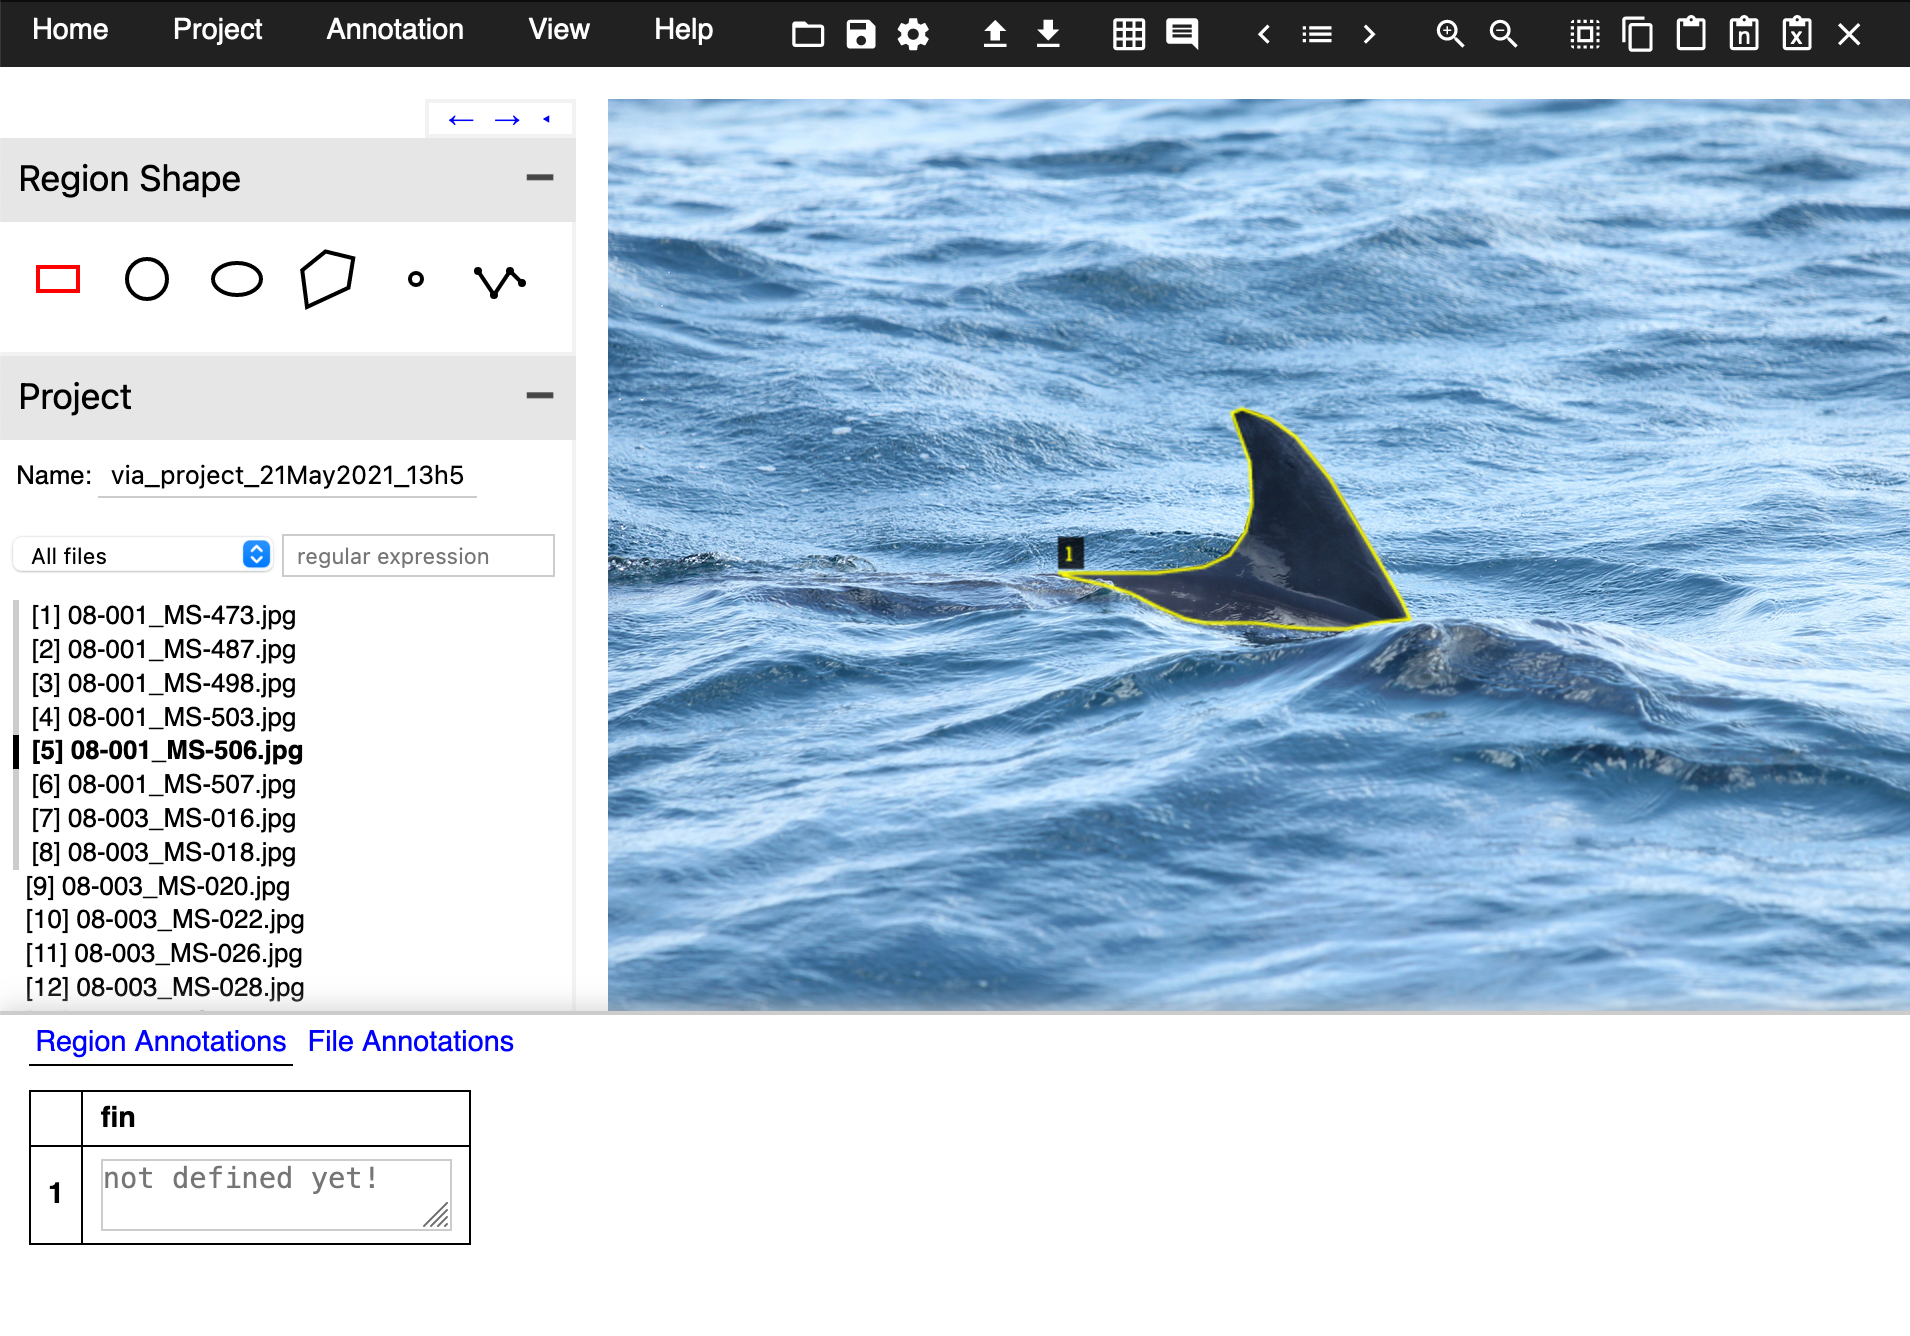
\includegraphics[scale=0.4]{Chapter3/figs/via-json-example-zanzibar-1.png}
	\end{center}
	\caption{An example image showing the labelling processes using VIA.
	}
	\label{fig:via-json-example-zanzibar}
\end{figure}

Once all 312 images had been labelled, it was then possible to create a train-test split. The 312 images were divided using an 80-20 split, where 80\% of the images are designated for training the Mask-RCNN model, known as the training set, and the remaining 20\% were held back for model evaluation, known as the test set. By evaluating on previously unseen data this affords researchers the ability to understand the generalisability of the trained model, mitigating overfitting. 

This newly created Zanzibar dataset would allow for prototyping to begin, determining the suitability of a Mask-RCNN based model for the task of a cetacean detector. The Zanzibar dataset was very similar in content to what would be expected from a dataset created from North Sea survey data once this had taken place and thus gave a good baseline for experimentation. 

\subsection{Transfer Learning}\label{ch:cetDet,sec:initialTesting,sub:transferLearning}

Whilst the Zanzibar dataset provides experimental data similar to that which the Mask-RCNN model will be required to process, the amount of data is extremely small. Deep learning models often require thousands of images when training to produce generalisable and accurate models. As such, this dataset alone would not be enough to train the cetacean detector. One way to fix this issue would be to locate more photo-id data. However, little extra data was readily available from the Marine MEGAfauna Lab, and data from other labs would require a large amount of effort to obtain. Cetacean catalogues are closely guarded by conversation labs due to the large amount of effort required to obtain them. Second, any further data collected would also need to be labelled and incorporated into the now existing dataset, which again would require significant time and effort. These issues rendered the prospect of expanding the Zanzibar dataset unachievable in the time required. 

Another available fix for this issue is the concept of transfer learning. This is a technique whereby models trained to perform one task are repurposed to aid in a second, usually more specialised task. These initial models have typically been trained on large generalised datasets such as ImageNet \cite{deng_imagenet:_2009} or Microsoft's Common Objects in Context, more commonly known as MSCOCO \cite{lin_microsoft_2014}. These datasets often contain hundreds of thousands of images covering a large number of classes, which make them perfect for the task of transfer learning. 

By first training a model on these large datasets, the model is able to learn the basics of image understanding, for example the concept of basic shapes and colour, allowing for the development of a generic visual understanding model. By utilising these models, we effectively provide our own model with a head-start in its learning process, there is no need to utilise the small amount of data available in the Zanzibar dataset for low level learning; it can instead be saved for allowing the model to understand and generalise to the domain specific task, such as cetacean detection. For a more in-depth analysis of transfer learning, see Pan \textit{et al.} \cite{pan_survey_2010}.

Training a neural network, or model, is extremely computationally and time expensive due to the large dataset sizes used. As such, many models suitable for transfer learning can be obtained in a pre-trained state. These pre-trained models are hosted by model zoos, which provide frozen model weight files in a format which allow for transfer learning to take place through a process known as fine-tuning. Here, a model from the zoo is downloaded and \textit{n}-number of deeper layers are unfrozen. Next, additional layers are added to the model which perform the domain specific task. The unfrozen and additional layers are then trained on the domain specific task, allowing for the fine-tuning of the higher-level feature extraction. 

\subsection{Utilising Transfer Learning to Train the Mask-RCNN}\label{ch:cetDet,sec:initialTesting,sub:transferLearningforTheDetector}

The use of transfer learning can be easily adapted for the training of the cetacean detector for use with the Zanzibar dataset, achieved directly through Tensorflow. First, a backbone model architecture is chosen. For the cetacean detector, it was decided that a ResNet50 backbone would be utilised. Matterport's Mask-RCNN implementation allows for the use of a ResNet50 or ResNet101 backbone, both standard variants of ResNet which are 50 and 101 layers deep respectively \cite{he_deep_2015}. ResNet50 was chosen over ResNet101 as during initial experimentation with the Matterport provided tutorial data, no significant improvement in accuracy was achieved using the deeper 101 layer model although a significant increase in training time was observed.

Once a backbone architecture was chosen, it can then be loaded into Tensorflow. Next, the pre-trained model weights are downloaded from the model zoo. These weights denote the strength of the connections between the model's layers. In the case of a model being trained from scratch without transfer learning, the weights of each layer are randomly initialised and then manipulated through backpropagation to achieve a desired model output. 

In transfer learning however, the model's starting weights are not initialised randomly. Instead, the weights of the trained network hosted on the model zoo are used as a starting point. This replicates the final state of the model trained on the larger dataset. 

As previously mentioned, there are multiple different models available in the zoo, all trained on a large variety of benchmark datasets. Each dataset produces a model with different final trained weights. Before applying transfer learning to the ResNet50 architecture chosen it is important to make an informed decision as to which benchmark dataset the model should be initialised from. 

For this project it was decided that the ResNet50 weights trained on MSCOCO \cite{lin_microsoft_2014} would be utilised. This was due to the fact that MSCOCO is primarily an instance segmentation dataset, and thus one of the most appropriate to use for transfer learning to another instance segmentation task. The use of MSCOCO for pre-training on Mask-RCNN has in recent years been well documented in literature for a variety of tasks \cite{yu_fruit_2019, couteaux_automatic_2019, fujita_fine-tuned_2020}. 

When utilising an MSCOCO pre-trained architecture for a Mask-RCNN based task, it is important to note that certain layers must be excluded when loading in the pre-trained weights as these are only utilised in Mask-RCNN models, such as those which deal with the per-pixel masks. This is because these layers require the same number of neurons as dataset classes, similar to a fully connected layer. If the MSCOCO weights were utilised at these final layers for the task at hand there would be a mismatch between the number of classes in MSCOCO, 80, and in the Zanzibar dataset, 1 (plus \texttt{background}).

Once the backbone architecture has been loaded with pre-trained weights, the total number of layers to fine-tune must be decided. This can be considered similar to a hyperparameter, as it must be chosen at run time by the user. Whilst any number of the layers can be chosen for fine-tuning, only the model heads are selected. These are layers required for the Region Proposal Network, the pixel classification, and masking layers of the model. For the purposes of hyperparameter tuning, whether the model weights are randomly initialised or loaded from a pre-trained model can be selected.

\subsection{Data Augmentation}\label{ch:cetDet,sec:initialTesting,sub:dataaugmentation}

As well as transfer learning the use of data augmentation was also explored to help mitigate the issue of dataset size. This technique allows for datasets to be artificially expanded by performing random perturbations to each data point which are then automatically class labelled the same as the original input. Figure \ref{fig:data-aug-examples} shows examples of data augmentations found in literature.

\begin{figure}[h]
	\begin{center}
		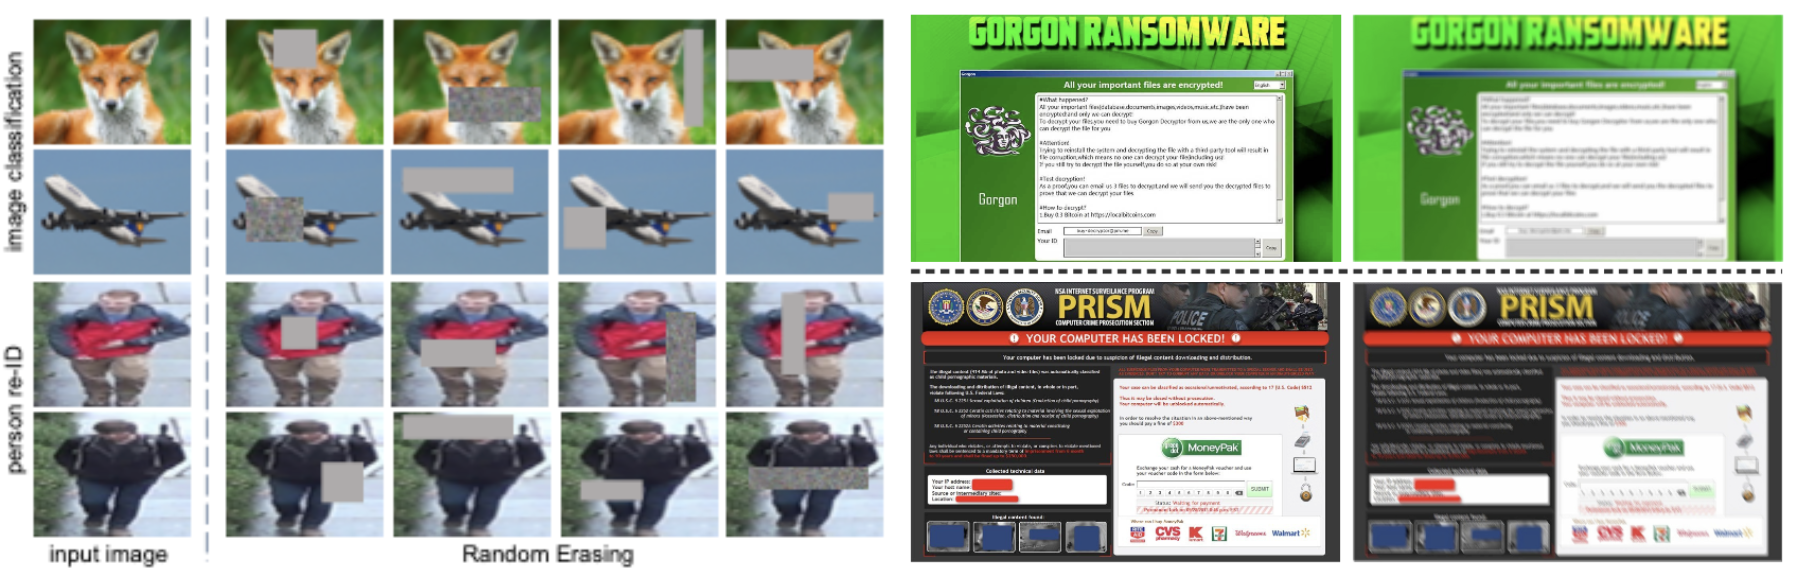
\includegraphics[scale=0.45]{Chapter3/figs/data-augs.png}
	\end{center}
	\caption{Examples of data augmentations found in literature.}{Examples of data augmentations found in literature. Left: Randomly erasing parts of images, from Zhong \textit{et al}. \cite{zhong_random_2017}. Right: Augmentations to simulate screenshot capture. Defocus blur (top), motion blur (bottom) from Atapour-Abarghouei \textit{et al}. \cite{atapour-abarghouei_kings_2019}.}
	\label{fig:data-aug-examples}
\end{figure}

When augmenting data it is extremely important to understand a dataset's problem domain to ensure that any transformations are realistic and expose the model trained to data which, whilst not present in the dataset before augmentation, could still reasonably expected to be seen by the model when deployed. Further, augmentation must only occur on the training data and not the test data. This is in contrast to preprocessing techniques such as resizing, which must occur to all data points. 

As the Zanzibar data contains relatively few images, it is a prime candidate for data augmentation. This can be performed in one of two ways; in either an offline or an online manner. In offline data augmentation, the entire train split is augmented before the images are passed to the model, occurring as a preprocessing step. This is extremely useful for very small datasets where the number of examples needs to be increased before the model can begin training, or if training time is a concern. The major issue with offline augmentations however is that, because the data is perturbed and then passed to the model, offline augmentation produces a fixed number of augmented images. 

This can be solved with online augmentation, which occurs in real-time as the model trains. The model is passed the original, unperturbed data which is then augmented during each training batch. This allows for the model to see a potentially unlimited number of `new' images, as each input image is randomly perturbed before being used for training. Once training on the batch has been completed, the augmented images are discarded and new perturbations performed. As such online augmentation is, if possible, greatly preferred and allows for a much higher chance of model generalisation. 

Whilst the Zanzibar dataset is small compared to others used for deep learning, it is large enough to allow for online augmentation. In order to begin testing the effect of data augmentation on the Mask-RCNN training process, two different augmentation strategies were created which contained unique workflows. 

The first strategy, \textit{aug1}, selected between zero and three of the following perturbations: (1) \textit{horizontal flip}: flip the image horizontally with a probability of 0.5, (2) \textit{vertical flip}: flip the image vertically with a probability of 0.5, (3) \textit{rotation}: rotate the image either 90, 180, or 270 degrees each with equal probability of occurring, (4) \textit{scaling}: scale the image between 80\% and 120\% on both axis independent of each other, (5) \textit{brightness}: multiply all pixels in the image with a random value between 0.8 and 1.5, (6) \textit{Gaussian blur}: blur the image with a Gaussian kernel with radius randomly assigned between 0 and  5. 

The second strategy, \textit{aug2}, was more complex, performing the following perturbations in a sequentially random order on 67\% of the images only: (1) \textit{horizontal flip}: flip the image horizontally with a probability of 0.5, (2) \textit{cropping}: crop each side of the image randomly between 0\% and 10\% of the total side length, (3) \textit{Gaussian blur}: blur the image with a Gaussian kernel with radius randomly assigned between 0 and 2.5, with a probability of blurring of 0.5, (4) \textit{contrast}: strengthen or weaken the contrast of the image by a random factor between 0.75 and 1.5, (5) \textit{additive Gaussian noise}: sample the noise per channel - adding noise to the colour of the pixels, (6) \textit{brightness}: multiply all pixels in the image with a random value between 0.8 and 1.2, (7) \textit{scaling}: scale the image between 80\% and 120\% on both axis independent of each other, (8) \textit{rotation}: rotate the image randomly between -180 and 180 degrees. 

The use of two augmenters allowed for evaluation on whether a simple or more complex augmentation strategy would be appropriate for this use case. By using multiple augmenters we can treat them as a hyperparameter of model training, allowing the augmenter chosen to be added to the search space.

\section{Mask-RCNN Model Selection}\label{ch:cetDet,sec:ModelSelection}

When training a Mask-RCNN model there are a large range of hyperparameters, or user defined values, which must be set before training can occur. These hyperparameters each have influence on the final model's performance, and can be broken down into two subgroups; detection hyperparameters influence the output of the model, and training hyperparameters which influence the training of the model. Thankfully most deep learning frameworks provide default values for most, if not all hyperparameters. These default values are known to work well regardless of dataset or task, and so many have been used when training the Mask-RCNN. Some hyperparameters however can have a large effect on the final model and so an exploration of the optimal value for these has been undertaken with the goal of producing the optimal overall model for the task of cetacean detection, both on the Zanzibar dataset and on other similar datasets. 

\subsection{Detection Hyperparameters}\label{ch:cetDet,sec:ModelSelection,sub:DetectionHyperparameters}
 
 With regards to the detection hyperparameters, only the minimum confidence of the model was changed from the default of 0.7 to 0.9. This was changed as during initial trials it was found models trained on the Zanzibar data would often produce a high number of false positives (for example detecting a wave as a fin) or create duplicate detections (one fin detected twice). By increasing the minimum confidence of the model to 0.9, we increase the threshold at which the model returns a detection to 90\%, or in other words for every detection the model must be 90\% sure that the detection is actually a fin before notifying the user. This reduced both the false positive rate and duplicate detection rate of the model. As example of this can be seen in Figure \ref{fig:min-conf}. Note how in the left image more detections are present than in the right image, however the extra detections are either part of an existing detection (yellow) or do not contain enough fin to identify the individual (red).
 
\begin{figure}[h]
	\begin{center}
		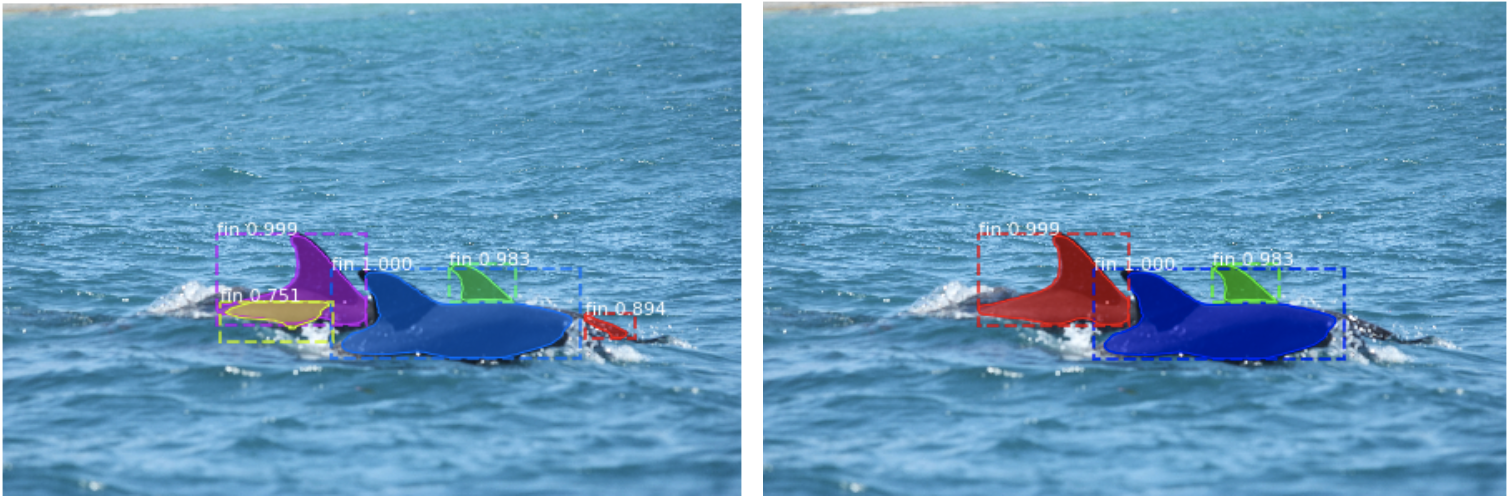
\includegraphics[scale=0.55]{Chapter3/figs/min-conf-eg.png}
	\end{center}
	\caption{An example image showing the effect of minimum detection confidence thresholding in Mask-RCNN detections. Left: A threshold of 0.7. Right: A threshold of 0.9.}
	\label{fig:min-conf}
\end{figure}
 
 
\subsection{Training Hyperparameters}\label{ch:cetDet,sec:ModelSelection,sub:TrainingHyperparameters}

The vast majority of hyperparameters are those which influence the training process. Selection of the optimal hyperparameters is an extremely computationally and time expensive task, as the optimal values of the hyperparameters are not known before training begins. Indeed, even after training has finished and a model which produces satisfactory results has been found there is no guarantee that the hyperparameters of this model are the best, just that they were the best found so far. 

As such, in order to determine the best hyperparameters for a given model and task, the search space of all possible hyperparameters must be searched. This is infeasible due to time and resource constraints however, and as such techniques such as grid searching was performed. During a grid search, each of the possible hyperparameters will have a range of values defined. A model is then trained using the data and each combination of defined hyperparameter values. Once each model has been trained, they are then evaluated to determine the best hyperparameters. In some cases an acceptable model will be found during the initial grid search, however this may not be the case. In this situation the previous grid search may not be useless, as it may provide insight into how to refine the search space to increase the chances of an acceptable model being trained. This process of finding the optimal hyperparameters for the model is known as hyperparameter tuning. 

\subsubsection{Learning Rate Scheduling \& Optimisers}\label{ch:cetDet,sec:ModelSelection,sub:TrainingHyperparameters,subsub:learningRateOptimisers}
One of the most important hyperparameters to tune is the learning rate, which dictates how much the weights of the model should change in response to the estimated error calculated during backpropagation. If the learning rate is too large this will lead to an unstable training process whereby gradient descent can never reach the minimum value but rather bounce either side of it. If the learning rate is set too small the training process will take an extremely long time to converge. 

In order to help the model reach its optimal minima in a reasonable time, the learning rate can be scheduled using a scheduler. These allow for the learning rate to be modified when some criteria is met, such as after a set number of epochs, allowing for larger weight changes initially for fast training before reducing the descent steps as time goes on, decreasing the chance of gradient descent jumping over the minima.

As well as learning rate schedulers, adaptive rate optimisers can also be used. These optimisers provide an alternative to SGD and are capable of adapting to the dataset it is given and the current training process, changing the learning rate without a defined schedule. This often allows for a more optimised and efficient training process when compared to using SGD, as discussed in Section \ref{ch:Background,sec:DLIntro,sub:stochasticgradientdescent}. During hyperparameter tuning of the Mask-RCNN, two optimisers were chosen for evaluation. 

The first, SGD with restarts (SGDR) \cite{loshchilov_sgdr:_2016} allows for decreases in the learning rate through a process known as cosine annealing, whereby the decrease follows a cosine waveform. This results in a high starting learning rate allowing for a fast approach to a local minima before reducing the rate as the number of epochs increases to prevent a jump over the minima, similarly to how a scheduler works. However it may not be the case that this local minima is the global minima, the lowest possible point in the space. Due to cosine annealing it would not be possible to leave the local minima, the learning rate needs to be increased again to allow for this. As such the learning rate is \textit{restarted}, or increased back to its maximum, to allow for the training process to jump out of the local minima; if it is indeed the case that this local minima is also the global minima then the training process will return to the point it was at before the restart, however if the local minima was not the global minima, the restart will allow for the training process to leave the sub-optimal minima it previously found. 

The second learning rate optimisation explored during hyperparameter tuning is Adam, or adaptive moment estimation. This optimiser is extremely popular in the world of deep learning \cite{karpathy_peek_2017}, capable of achieving impressive results in relatively short training times. This is possible through the use of one learning rate for each model weight, in contrast to the singular learning rate for the whole model as seen in SGD or SGDR. Adam also utilises parts of other optimisers such as AdaGrad \cite{duchi_adaptive_2011} and RMSProp \cite{tieleman_lecture_2012} to allow the optimiser to work well with both sparse and noisy data. For a complete breakdown of the inner workings of Adam, see Kingma \textit{et al}. \cite{kingma_adam:_2014}. 

\subsubsection{Weight Decay}\label{ch:cetDet,sec:ModelSelection,sub:TrainingHyperparameters,subsub:WeightDecay}

The goal of neural network development is to utilise the training data in such a way that the resulting generated model performs well on unseen data. In order for this to be achieved our model must be generalisable, having learnt enough from the training data to perform well at the given task but not having learnt so well that it is unable to perform adequately on unseen data. If a model fails to generalise, it is said to have overfitted the data. For example lets say we wish to develop a cat detector, a model which given an input image will tell you if there is a cat present. However, we only train our model on images with white cats in them. The model trains well, and is always able to tell you if there is a cat in the images it sees during training. When deployed, the model fails to identify any images containing black cats - the model has learnt the training data too well and believes cats can only be white; the model has overfitted. 

There are many different techniques to reduce overfitting in neural networks, one of the easiest is to simply collect more training data. As previously mentioned, due to how closely guarded cetacean photo-id catalogue data is and how expensive it is to collect, this was not possible. As such, the use of weight decay was explored during hyperparameter tuning. Weight decay is a regularisation technique which allows the model training to be penalised in proportion to the size of its weights. This incentivises the training process to keep the weights small, which has been shown to improve generalisation to unseen data \cite{krogh_simple_1991}. As the Zanzibar dataset is comparability small compared to the usual size of datasets for this task, allowing the model to generalise well using small amounts of data is extremely important.

\subsubsection{RPN Anchor Scales}\label{ch:cetDet,sec:ModelSelection,sub:TrainingHyperparameters,subsub:RPNAnchorScales}

As discussed in Section \ref{ch:Background,sec:objectDetection,sub:RPN}, Region Proposal Networks (RPNs) can be utilised in object detection due to their ability to determine potential regions of interest (RoIs) in the image, known as anchors. These anchors are then classified as either \texttt{background} or of a learnable class, such as \texttt{dolphin}. To allow the RPN to be object-size invariant, anchor scales are utilised. These scales, provided as a list of values which correspond to the square anchor side in pixels, determine what sizes the RoIs proposed by the RPN should be. For example, let's say an anchor scale of \texttt{[32]} is passed to the RPN, this would mean that all RoIs proposed by the RPN would be of size 32x32 pixels. The anchor scale provided to the RPN can be considered a hyperparameter as the best scales for the RPN to allow for the detection of objects regardless of their size must be determined. 

\subsection{Hyperparameter Tuning via a Grid Search}\label{ch:cetDet,sec:ModelSelection,sub:HyperparameterTuning}

Although only a few hyperparameters have been chosen to tune, the size of the possible search space to evaluate is still extremely large. As mentioned previously, it is not feasible both from a time and resource perspective to evaluate the entire space and find the truly optimal value for each hyperparameter. Instead the search space is discretised using a grid search, for each hyperparameter a subset of possible values is selected. Each combination of hyperparameter values is then evaluated to determine which set of values produces a satisfactory model. 

The list of possible hyperparameter combinations and model name, determined by the datetime value at the start of the model's training run, can be seen in Table \ref{tab:MaskRCNNHyperparamTuningGridSearch}. This reduced hyperparameter tuning run still required significant amount of time and resources, running over three NC12 Microsoft Azure VMs, each with two Tesla K80 GPUs, taking approximately one week to complete the grid search producing a total of 50 models. Model runs were split between the VMs based on augmentation strategy with one VM running only \textit{aug1}, the other \textit{aug2}, and the final with no augmentation strategy. It should be noted here that this computational and time expense would most likely be reduced should the images used to train the Mask-RCNN not be so large, although the reasons for this decision are discussed in Section \ref{ch:cetDet,sec:requirements,sub:technical}.

\begin{table}[!ht]
	\tiny
	\begin{adjustbox}{width=\columnwidth, center}
		\begin{tabular}{cccccc}
			\toprule
			Model Name & Weight Decay &        RPN Anchor Scales & Optimiser & Augmentation Strategy & Pre-trained on MSCOCO? \\
			\midrule
			20190829T1458 &         0.01 &   (16, 32, 64, 128, 256) &      Adam &                  aug1 &                  True \\
			20190829T2020 &         0.01 &   (16, 32, 64, 128, 256) &      Adam &                  aug2 &                  True \\
			20190830T0145 &         0.01 &   (16, 32, 64, 128, 256) &      Adam &                  None &                  True \\
			20190830T0714 &         0.01 &   (16, 32, 64, 128, 256) &      Adam &                  aug1 &                   False \\
			20190830T1443 &         0.01 &   (16, 32, 64, 128, 256) &      Adam &                  aug2 &                   False \\
			20190830T2019 &         0.01 &   (16, 32, 64, 128, 256) &      Adam &                  None &                   False \\
			20190902T0946 &         0.01 &   (16, 32, 64, 128, 256) &      SGDR &                  aug1 &                  True \\
			20190904T2004 &         0.01 &   (16, 32, 64, 128, 256) &      SGDR &                  None &                  True \\
			20190905T1813 &        0.001 &  (32, 64, 128, 256, 512) &      SGDR &                  aug1 &                  True \\
			20190905T1826 &         0.01 &   (16, 32, 64, 128, 256) &      SGDR &                  aug2 &                  True \\
			20190905T2202 &        0.001 &  (32, 64, 128, 256, 512) &      Adam &                  None &                  True \\
			20190905T2336 &        0.001 &  (32, 64, 128, 256, 512) &      Adam &                  aug1 &                  True \\
			20190906T0332 &        0.001 &  (32, 64, 128, 256, 512) &      SGDR &                  None &                  True \\
			20190906T0851 &         0.01 &  (32, 64, 128, 256, 512) &      Adam &                  None &                  True \\
			20190907T0932 &        0.001 &   (16, 32, 64, 128, 256) &      Adam &                  aug1 &                  True \\
			20190907T0933 &       0.0001 &  (32, 64, 128, 256, 512) &      Adam &                  aug2 &                   False \\
			20190907T0934 &         0.01 &  (32, 64, 128, 256, 512) &      SGDR &                  None &                  False \\
			20190907T1451 &        0.001 &   (16, 32, 64, 128, 256) &      Adam &                  None &                  True \\
			20190907T1500 &       0.0001 &  (32, 64, 128, 256, 512) &      Adam &                  aug1 &                   False \\
			20190907T1545 &         0.01 &  (32, 64, 128, 256, 512) &      Adam &                  aug2 &                   False \\
			20190907T2026 &       0.0001 &  (32, 64, 128, 256, 512) &      SGDR &                  None &                  True \\
			20190907T2126 &        0.001 &   (16, 32, 64, 128, 256) &      Adam &                  aug1 &                   False \\
			20190907T2215 &        0.001 &   (16, 32, 64, 128, 256) &      SGDR &                  aug2 &                  True \\
			20190908T0202 &       0.0001 &   (16, 32, 64, 128, 256) &      Adam &                  None &                  True \\
			20190908T0352 &         0.01 &  (32, 64, 128, 256, 512) &      Adam &                  aug2 &                  True \\
			20190908T0417 &       0.0001 &  (32, 64, 128, 256, 512) &      Adam &                  aug1 &                  True \\
			20190908T0957 &       0.0001 &  (32, 64, 128, 256, 512) &      Adam &                  None &                   False \\
			20190908T1102 &       0.0001 &  (32, 64, 128, 256, 512) &      Adam &                  aug2 &                  False \\
			20190908T1204 &        0.001 &   (16, 32, 64, 128, 256) &      SGDR &                  aug1 &                  True \\
			20190908T1939 &        0.001 &   (16, 32, 64, 128, 256) &      Adam &                  aug2 &                   False \\
			20190908T2043 &       0.0001 &  (32, 64, 128, 256, 512) &      SGDR &                  aug1 &                  True \\
			20190908T2139 &       0.0001 &   (16, 32, 64, 128, 256) &      Adam &                  None &                   False \\
			20190909T0723 &       0.0001 &   (16, 32, 64, 128, 256) &      Adam &                  aug1 &                   False \\
			20190911T1922 &         0.01 &   (16, 32, 64, 128, 256) &      Adam &                  aug2 &                   False \\
			20190912T0045 &       0.0001 &   (16, 32, 64, 128, 256) &      Adam &                  aug2 &                   False \\
			20190912T0608 &       0.0001 &   (16, 32, 64, 128, 256) &      SGDR &                  aug1 &                  True \\
			20191101T1633 &       0.0001 &  (32, 64, 128, 256, 512) &      SGDR &                  aug2 &                  True \\
			20191101T2104 &        0.001 &     (8, 16, 32, 64, 128) &      SGDR &                  aug2 &                  True \\
			20191102T0140 &         0.01 &  (32, 64, 128, 256, 512) &      SGDR &                  aug1 &                  True \\
			20191102T0615 &         0.01 &     (8, 16, 32, 64, 128) &      SGDR &                  aug2 &                  True \\
			20191102T1051 &       0.0001 &   (16, 32, 64, 128, 256) &      SGDR &                  None &                  False \\
			20191102T1528 &        0.001 &  (32, 64, 128, 256, 512) &      SGDR &                  aug2 &                  True \\
			20191102T2006 &       0.0001 &     (8, 16, 32, 64, 128) &      SGDR &                  aug2 &                  True \\
			20191103T0044 &       0.0001 &     (8, 16, 32, 64, 128) &      SGDR &                  aug1 &                  True \\
			20191103T0520 &        0.001 &     (8, 16, 32, 64, 128) &      SGDR &                  None &                  True \\
			20191103T0959 &         0.01 &  (32, 64, 128, 256, 512) &      SGDR &                  aug2 &                  True \\
			20191103T1441 &       0.0001 &     (8, 16, 32, 64, 128) &      SGDR &                  None &                  True \\
			20191103T1921 &       0.0001 &   (16, 32, 64, 128, 256) &      SGDR &                  aug2 &                  True \\
			20191104T0011 &        0.001 &     (8, 16, 32, 64, 128) &      SGDR &                  aug1 &                  True \\
			20191104T0450 &         0.01 &     (8, 16, 32, 64, 128) &      SGDR &                  aug1 &                  True \\
			\bottomrule
		\end{tabular}
	\end{adjustbox}
	\caption{Hyperparameter values used for each grid search run when training the Mask-RCNN model on the Zanzibar data.}\label{tab:MaskRCNNHyperparamTuningGridSearch}
\end{table}

\subsection{Model Selection Based on Grid Search}\label{ch:cetDet,sec:ModelSelection,sub:ModelSelectionBasedOnGridSearch}

Once a grid search has been performed, the results can then be evaluated to determine if a suitable model had been found using the test set. All models trained were evaluated using MSCOCO's Mean Average Precision metric\footnote{COCO mAP Definition: \href{https://cocodataset.org/\#detection-eval}{cocodataset.org/\#detection-eval}}, a commonly used metric for segmentation tasks. This metric, commonly written as mAP@IOU[0.5:0.95], calculates precision-recall graphs for each dataset class at incremental IOU levels, from 0.5 to 0.95 in 0.05 steps. Once each class' precision-recall graph for a given IOU threshold has been calculated, the mean of these values is derived giving an overall mean average precision score for all classes at a given IOU threshold; these thresholds are explained in more detail in Section \ref{ch:Background,sec:semanticSegmentation}.

By evaluating over multiple thresholds the models can then be compared and their performance more easily understood and ranked, as well as allow for the determination of an acceptable loss in IOU overlap. For example if all models were evaluated using mAP@IOU[0.5] only, it may be the case that all models achieve a similar high score, making it difficult to determine which model will be best for the task. However if too high a threshold is used, for example mAPIOU[0.95], it is unlikely that any model will achieve a high score as this would require constant near pixel perfect detection. 

Figure \ref{fig:mAP-graph} shows a visualisation of the mAP@IOU[0.5:0.95] scores for all models trained in the grid search, the raw scores can be seen in Appendix \ref{app:mAPScoresGridSearch}. At mAP@IOU[0.5] there is a large gap in model performance with model 20190830T1443 having the lowest mAP@IOU[0.5] of 0.73 and model 20190905T1813 having the highest at 0.94. This shows that the combination of hyperparameter values provided to the model before training have a significant effect on the model's overall performance, although even the lowest score here is still high. 

At mAP@IOU[0.75], whereby detections would overlap with 75\% of pixels in the ground truth mask, the minimum model performance has dropped significantly with model 20190830T071 achieving a score of 0.49. The highest score at this threshold is model 20191102T0140 with a score of 0.81; this model achieved an map@IOU[0.5] score of 0.92, only two percentage points behind the best model at that threshold. This again shows the need for hyperparameter tuning when selecting models, as they are shown here to have a significant effect on how well the models perform at higher thresholds.

This effect is even greater when comparing map@IOU[0.85] scores, with the worst performing model, 20190830T0714,  achieving a score of just 0.17 whilst the best model, 20190902T0946, achieves a score of 0.50, a difference of 33\%. Model performance drops significantly at the highest threshold with four models achieving an mAP@IOU[0.95] score of 0.016, with most models achieving a score of 0.0. This is to be expected however as it would be highly unlikely that any model, regardless of hyperparameters, would be able to perform near perfect pixel level detections on the test set data. 

\begin{figure}[h]
	\begin{center}
		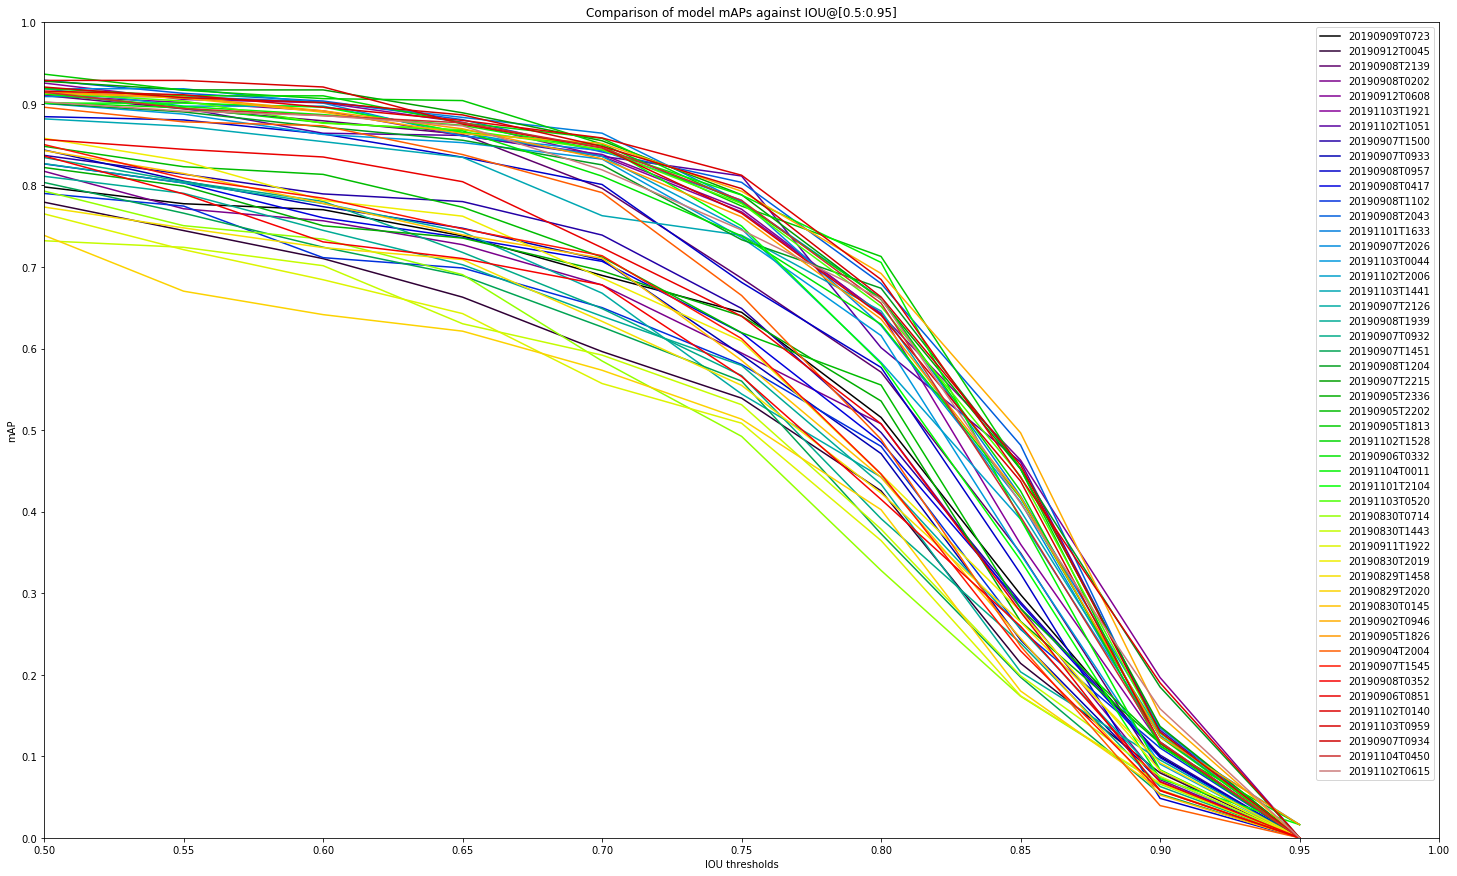
\includegraphics[scale=0.33]{Chapter3/figs/comparison_graph_all_diff_colours.png}
	\end{center}
	\caption{mAP@IOU[0.5:0.95] scores for all models train in the Mask-RCNN Zanzibar dataset grid search. See Table \ref{tab:MaskRCNNHyperparamTuningGridSearch} for each model's hyperparameters.}
	\label{fig:mAP-graph}
\end{figure}

Whilst Figure \ref{fig:mAP-graph} provides some indication of overall model training, using it to determine the most appropriate model for the task at hand is difficult given the number of models trained. To achieve this, the list of models was reduced to only those which achieved the best mAP@IOU[0.5, 0.75, 0.85] scores. The thresholds 0.5 and 0.75 were chosen as these are often cited in segmentation literature \cite{bolya_190402689_2019, wang_solov2_2020, tian_fcos_2019}. The 0.85 threshold was chosen as some models trained still achieve impressive results here, allowing for more model filtering. Further, the pixel-wise detections of fins is required to filter as much background noise as possible and so finding high performing models at top thresholds is important.

When filtering, the top five performing models at each threshold were extracted and then combined into one list. If a model  achieved top five ranking at multiple thresholds it was only included in the list once, resulting in a list of ten best performing models. The mAP@IOU[0.5, 0.75, 0.85] scores for these best performing models can be seen in Figure \ref{fig:mAP-best-models-bar-chart}.

\begin{figure}[h]
	\begin{center}
		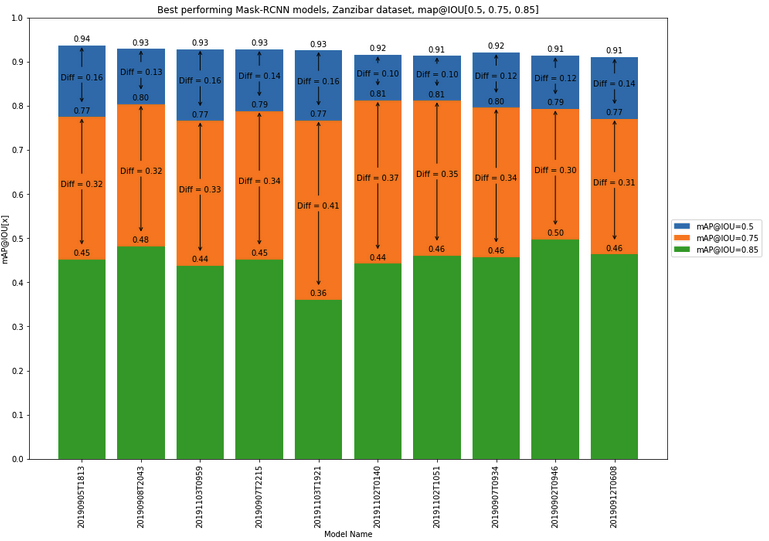
\includegraphics[scale=0.6]{Chapter3/figs/mask-RCNN-model-bar-chart.png}
	\end{center}
	\caption{mAP@IOU[0.5, 0.75, 0.85] scores for the best performing Mask-RCNN models trained on the Zanzibar dataset. See Table \ref{tab:MaskRCNNHyperparamTuningGridSearch} for each model's hyperparameters.}
	\label{fig:mAP-best-models-bar-chart}
\end{figure}

When deciding on which model hyperparameters are best for the task of cetacean segmentation, it is important to find a model with a high mAP@IOU[0.85] score. As the model will be used to perform segmentation before fine-grained classification, it is important the model is capable of removing as much background from the inputted image as possible. Any background included in the segmentation may adversely effect the photo-id process. Using this as criteria, model 20190902T0946 was selected as the best performing model. The model achieves an mAP@IOU[0.85] score of 0.5, an excellent result given the difficulty of the segmentation task. The model also performs well at the other evaluation thresholds, achieving mAP@IOU[0.5, 0.75] scores of 0.91 and 0.79 respectively. These scores verify the model is capable of segmenting cetacean fins from background with as little noise being included in the segmentation mask as possible.

An interesting point to note here is that 20190902T0946 did not achieve the highest mAP@IOU[0.5, 0.75] scores. As previously mentioned, these thresholds are often the ones included in segmentation literature to evaluate model performance. If just these thresholds were used for model selection, 20190902T0946 would not have been chosen. This highlights the need to select models based on metrics which make sense for the task at hand. As the model is required to remove as much background noise as possible, using a high threshold for evaluation makes sense. Thresholds higher than 0.85 were not utilised due to the low performance of all models at this threshold, although 20190902T0946 also achieves one of the best mAP@IOU[0.9] score of 0.150. Only one model, 20191102T0615 achieves a better score at this threshold, 0.158, however this model achieves lower performance at the chosen evaluation thresholds of 0.5, 0.75, and 0.85.

\subsection{An Evaluation of Optimal Model Hyperparameters}\label{ch:cetDet,sec:ModelSelection,sub:OptimalHyperparameters}

As discussed in Section \ref{ch:cetDet,sec:ModelSelection,sub:ModelSelectionBasedOnGridSearch} a filter of the trained Mask-RCNN models was performed to determine the best model hyperparameters for the task of cetacean instance segmentation, with model 20190902T0946 being selected. This model's hyperparameters, along with those of the other nine best performing models, can be seen in Table \ref{tab:best-mask-rcnn-models}.

\begin{table}[!ht]
	\tiny
	\begin{adjustbox}{width=\columnwidth, center}
		\begin{tabular}{cccccc}
			\toprule
			Model Name & Weight Decay &        RPN Anchor Scales & Optimiser & Augmentation Strategy & Pre-trained on MSCOCO? \\
			\midrule
				20190902T0946 &         0.01 &   (16, 32, 64, 128, 256) &      SGDR &                  aug1 &                  True \\
				20190905T1813 &        0.001 &  (32, 64, 128, 256, 512) &      SGDR &                  aug1 &                  True \\
				20190907T0934 &         0.01 &  (32, 64, 128, 256, 512) &      SGDR &                  None &                  True \\
				20190907T2215 &        0.001 &   (16, 32, 64, 128, 256) &      SGDR &                  aug2 &                  True \\
				20190908T2043 &       0.0001 &  (32, 64, 128, 256, 512) &      SGDR &                  aug1 &                  True \\
				20190912T0608 &       0.0001 &   (16, 32, 64, 128, 256) &      SGDR &                  aug1 &                  True \\
				20191102T0140 &         0.01 &  (32, 64, 128, 256, 512) &      SGDR &                  aug1 &                  True \\
				20191102T1051 &       0.0001 &   (16, 32, 64, 128, 256) &      SGDR &                  None &                  True \\
				20191103T0959 &         0.01 &  (32, 64, 128, 256, 512) &      SGDR &                  aug2 &                  True \\
				20191103T1921 &       0.0001 &   (16, 32, 64, 128, 256) &      SGDR &                  aug2 &                  True \\
			\bottomrule
		\end{tabular}
	\end{adjustbox}
	\caption{Hyperparameters of the best performing Mask-RCNN models on the Zanzibar dataset. Subset of Table \ref{tab:MaskRCNNHyperparamTuningGridSearch}.}
	\label{tab:best-mask-rcnn-models}
\end{table}

The hyperparameters of the best performing models provide an interesting insight into the training process. All ten of the models were trained using SGDR. This is interesting, as the current trend in deep learning network training is to utilise Adam \cite{karpathy_peek_2017}. Furthermore each model trained utilised transfer learning, with each model's parameters being initialised from a trained MSCOCO model provided by the model zoo. This highlights the need to utilise pre-trained models, especially cases where relativity small amounts of data are available to train a model from scratch. 

Half of the best models utilise the \textit{aug1} data augmentation strategy, defined in Section \ref{ch:cetDet,sec:initialTesting,sub:dataaugmentation}. The smallest RPN Anchor Scale, (8, 16, 32, 64, 128), has not been utilised by any of the best models, and the value of the weight decay hyperparameter is split between the three possible values. These splits highlight the need for a robust and in-depth hyperparameter search, as with the majority of hyperparameters searched no clear trend can be identified.

\subsection{Summary}\label{ch:cetDet,sec:ModelSelection,sub:Summary}

%Summary of the Chapter. It is possible to create an instance segmentation model which is capable of handling the technical and environmental challenges of cetacean detection. Through the use of transfer learning and a dataset that is extremely different to the target domain, as well as hyperparameter tuning, it is possible to create a Mask-RCNN based detector which achieves high mAP. This removes unneeded background from the images, and removes images outright which do not contain a dolphin. Discuss the need to test the system on bottlenose and white-beaked datasets, as well as the need to utilise the pixel level detections to segment the fin from the image for photo-id.



%%%%%%%%%%%%%%%%%%%
\nomenclature[z-CNN]{CNN}{Convolutional Neural Networks}
\nomenclature[z-CV]{CV}{Computer Vision}
\nomenclature[z-CPU]{CPU}{Central Processing Unit}
\nomenclature[z-GPU]{GPU}{Graphical Processing Unit}
\nomenclature[z-SGD]{SGD}{Stochastic Gradient Descent}
\nomenclature[z-ReLU]{ReLU}{Rectified Linear Unit}
\nomenclature[z-FCN]{FCN}{Fully Convolutional Network}
\nomenclature[z-RPN]{RPN}{Region Proposal Network}
\nomenclature[z-SGDR]{SGDR}{Stochastic Gradient Descent with Restarts}
\nomenclature[z-VM]{VM}{Virtual Machine}


% ********************************** Back Matter *******************************
% Backmatter should be commented out, if you are using appendices after References
\backmatter

% ********************************** Appendices ********************************

\begin{appendices} % Using appendices environment for more functunality
	
	% ******************************* Thesis Appendix A ********************************
\renewcommand{\thesubsection}{\Alph{subsection}} % Make subsections alpha for appendix
\titleformat{\chapter}[display]
{\normalfont\huge\bfseries}{\chaptertitlename\ \thechapter}{20pt}{\Huge} % Recreate the default Chapter sizing and spacing so we can edit it and put the Mask-RCNN table on the same page

% this alters "before" spacing (the second length argument) to 0, "after" to 20pt
\titlespacing*{\chapter}{0pt}{0pt}{20pt}
\chapter{Appendix} 
% this changes "before" spacing back to its default of 50pt
\titlespacing*{\chapter}{0pt}{50pt}{40pt}

\setcounter{subsection}{0} % Force a reset of the appendix subsection lettering

\subsection{mAP@IOU[0.5:0.95] Scores for Mask-RCNN Grid Search Models}\label{app:mAPScoresGridSearch}

\begin{table}[!ht]
\centering
	\resizebox{!}{.6\height}{
		\small
		\begin{tabular}{ccccccccccc}
			\toprule
			\multirow{2}{*}{\bfseries Model Name} & 
			\multicolumn{10}{c}{\bfseries mAP@IOU[$x$]}\\ \cmidrule(lr){2-11}
			&\bfseries 0.5&\bfseries 0.55&\bfseries 0.6&\bfseries 0.65&\bfseries 0.7&\bfseries 0.75&\bfseries 0.8&\bfseries 0.85&\bfseries 0.9&\bfseries 0.95\\ \midrule
			
			20190909T0723 &          0.798 &          0.778 &          0.770 &          0.738 &          0.690 &          0.644 &          0.516 &          0.298 &          0.099 &          0.000 \\
			20190912T0045 &          0.780 &          0.745 &          0.710 &          0.663 &          0.596 &          0.539 &          0.425 &          0.214 &          0.080 &          0.000 \\
			20190908T2139 &          0.910 &          0.894 &          0.879 &          0.863 &          0.797 &          0.686 &          0.571 &          0.349 &          0.082 &          0.000 \\
			20190908T0202 &          0.817 &          0.771 &          0.757 &          0.727 &          0.678 &          0.594 &          0.508 &          0.281 &          0.071 &          0.000 \\
			20190912T0608 &          0.910 &          0.902 &          0.892 &          0.861 &          0.838 &          0.771 &          0.642 &          0.463 &          0.197 &          0.000 \\
			20191103T1921 &          0.926 &          0.905 &          0.901 &          0.878 &          0.836 &          0.768 &          0.643 &          0.360 &          0.115 &          0.000 \\
			20191102T1051 &          0.914 &          0.895 &          0.864 &          0.861 &          0.836 &          0.812 &          0.601 &          0.461 &          0.132 &          0.000 \\
			20190907T1500 &          0.837 &          0.814 &          0.790 &          0.780 &          0.739 &          0.649 &          0.497 &          0.289 &          0.101 &          0.000 \\
			20190907T0933 &          0.844 &          0.805 &          0.774 &          0.748 &          0.709 &          0.592 &          0.471 &          0.243 &          0.069 &          0.000 \\
			20190908T0957 &          0.884 &          0.880 &          0.863 &          0.835 &          0.801 &          0.681 &          0.577 &          0.324 &          0.048 &          0.000 \\
			20190908T0417 &          0.827 &          0.803 &          0.760 &          0.736 &          0.707 &          0.619 &          0.485 &          0.287 &          0.098 &          0.000 \\
			20190908T1102 &          0.790 &          0.775 &          0.712 &          0.699 &          0.650 &          0.581 &          0.480 &          0.256 &          0.110 &          0.000 \\
			20190908T2043 &          0.929 &          0.913 &          0.904 &          0.881 &          0.841 &          0.804 &          0.680 &          0.482 &          0.126 &          0.000 \\
			20191101T1633 &          0.909 &          0.909 &          0.902 &          0.883 &          0.864 &          0.780 &          0.662 &          0.419 &          0.135 &          0.000 \\
			20190907T2026 &          0.919 &          0.919 &          0.901 &          0.861 &          0.843 &          0.782 &          0.628 &          0.412 &          0.118 &          0.000 \\
			20191103T0044 &          0.901 &          0.888 &          0.863 &          0.853 &          0.832 &          0.736 &          0.616 &          0.348 &          0.090 &          0.000 \\
			20191102T2006 &          0.919 &          0.897 &          0.897 &          0.865 &          0.836 &          0.747 &          0.583 &          0.391 &          0.125 &          0.016 \\
			20191103T1441 &          0.882 &          0.873 &          0.854 &          0.835 &          0.763 &          0.739 &          0.646 &          0.401 &          0.129 &          0.000 \\
			20190907T2126 &          0.827 &          0.803 &          0.778 &          0.743 &          0.668 &          0.544 &          0.442 &          0.257 &          0.075 &          0.000 \\
			20190908T1939 &          0.811 &          0.790 &          0.745 &          0.703 &          0.640 &          0.579 &          0.434 &          0.203 &          0.095 &          0.000 \\
			20190907T0932 &          0.834 &          0.805 &          0.780 &          0.718 &          0.649 &          0.567 &          0.391 &          0.239 &          0.063 &          0.000 \\
			20190907T1451 &          0.804 &          0.766 &          0.724 &          0.689 &          0.626 &          0.560 &          0.373 &          0.197 &          0.054 &          0.000 \\
			20190908T1204 &          0.901 &          0.890 &          0.872 &          0.855 &          0.825 &          0.733 &          0.674 &          0.453 &          0.185 &          0.000 \\
			20190907T2215 &          0.928 &          0.917 &          0.917 &          0.889 &          0.855 &          0.789 &          0.660 &          0.452 &          0.137 &          0.000 \\
			20190905T2336 &          0.822 &          0.799 &          0.751 &          0.736 &          0.695 &          0.640 &          0.536 &          0.265 &          0.116 &          0.000 \\
			20190905T2202 &          0.848 &          0.823 &          0.814 &          0.773 &          0.712 &          0.619 &          0.555 &          0.281 &          0.116 &          0.000 \\
			20190905T1813 &          0.937 &          0.917 &          0.907 &          0.904 &          0.851 &          0.775 &          0.713 &          0.452 &          0.113 &          0.000 \\
			20191102T1528 &          0.919 &          0.910 &          0.910 &          0.877 &          0.858 &          0.778 &          0.661 &          0.425 &          0.112 &          0.016 \\
			20190906T0332 &          0.902 &          0.895 &          0.877 &          0.867 &          0.811 &          0.738 &          0.630 &          0.417 &          0.124 &          0.000 \\
			20191104T0011 &          0.912 &          0.897 &          0.887 &          0.874 &          0.844 &          0.788 &          0.706 &          0.391 &          0.083 &          0.000 \\
			20191101T2104 &          0.901 &          0.901 &          0.896 &          0.865 &          0.849 &          0.750 &          0.582 &          0.340 &          0.072 &          0.016 \\
			20191103T0520 &          0.913 &          0.904 &          0.876 &          0.868 &          0.844 &          0.778 &          0.652 &          0.443 &          0.129 &          0.000 \\
			20190830T0714 &          0.793 &          0.751 &          0.734 &          0.691 &          0.585 &          0.492 &          0.328 &          0.174 &          0.066 &          0.000 \\
			20190830T1443 &          0.732 &          0.724 &          0.702 &          0.630 &          0.592 &          0.531 &          0.379 &          0.199 &          0.075 &          0.000 \\
			20190911T1922 &          0.765 &          0.721 &          0.684 &          0.643 &          0.557 &          0.508 &          0.365 &          0.174 &          0.067 &          0.000 \\
			20190830T2019 &          0.858 &          0.830 &          0.782 &          0.762 &          0.687 &          0.609 &          0.446 &          0.278 &          0.082 &          0.000 \\
			20190829T1458 &          0.774 &          0.748 &          0.724 &          0.709 &          0.633 &          0.555 &          0.423 &          0.265 &          0.092 &          0.000 \\
			20190829T2020 &          0.739 &          0.670 &          0.642 &          0.621 &          0.573 &          0.513 &          0.402 &          0.180 &          0.059 &          0.000 \\
			20190830T0145 &          0.843 &          0.815 &          0.778 &          0.739 &          0.711 &          0.586 &          0.442 &          0.245 &          0.052 &          0.000 \\
			20190902T0946 &          0.914 &          0.907 &          0.890 &          0.864 &          0.852 &          0.793 &          0.692 &          0.497 &          0.150 &          0.000 \\
			20190905T1826 &          0.915 &          0.909 &          0.892 &          0.869 &          0.833 &          0.762 &          0.636 &          0.418 &          0.124 &          0.016 \\
			20190904T2004 &          0.896 &          0.878 &          0.873 &          0.838 &          0.791 &          0.665 &          0.489 &          0.235 &          0.040 &          0.000 \\
			20190907T1545 &          0.850 &          0.809 &          0.784 &          0.747 &          0.714 &          0.612 &          0.446 &          0.229 &          0.058 &          0.000 \\
			20190908T0352 &          0.836 &          0.790 &          0.731 &          0.710 &          0.678 &          0.566 &          0.415 &          0.259 &          0.069 &          0.000 \\
			20190906T0851 &          0.856 &          0.844 &          0.835 &          0.805 &          0.724 &          0.640 &          0.508 &          0.277 &          0.058 &          0.000 \\
			20191102T0140 &          0.916 &          0.911 &          0.896 &          0.880 &          0.858 &          0.813 &          0.685 &          0.442 &          0.190 &          0.000 \\
			20191103T0959 &          0.929 &          0.929 &          0.921 &          0.875 &          0.846 &          0.766 &          0.641 &          0.437 &          0.117 &          0.000 \\
			20190907T0934 &          0.921 &          0.908 &          0.902 &          0.887 &          0.848 &          0.796 &          0.663 &          0.457 &          0.130 &          0.000 \\
			20191104T0450 &          0.915 &          0.894 &          0.886 &          0.877 &          0.846 &          0.782 &          0.656 &          0.394 &          0.118 &          0.000 \\
			20191102T0615 &          0.902 &          0.891 &          0.886 &          0.873 &          0.819 &          0.745 &          0.661 &          0.410 &          0.158 &          0.000 \\
			\bottomrule
		\end{tabular}}
	\caption{mAP@IOU[0.5:0.95] scores for each Mask-RCNN model trained in the Zanzibar dataset grid search. See Section \ref{ch:cetDet,sec:ModelSelection,sub:HyperparameterTuning} for model hyperparameters.}
\end{table}






\end{appendices}

% ********************************** Bibliography ******************************
\begin{spacing}{0.9}

% To use the conventional natbib style referencing
% Bibliography style previews: http://nodonn.tipido.net/bibstyle.php

\bibliographystyle{apalike}
%\bibliographystyle{plainnat} % use this to have URLs listed in References
\cleardoublepage
\bibliography{References/references} % Path to your References.bib file

% If you would like to use BibLaTeX for your references, pass `custombib' as
% an option in the document class. The location of 'reference.bib' should be
% specified in the preamble.tex file in the custombib section.
% Comment out the lines related to natbib above and uncomment the following
%line.

%\printbibliography[heading=bibintoc, title={References}]


\end{spacing}



% *************************************** Index ********************************
%\printthesisindex % If index is present

\end{document}
